
\documentclass[pdftex,a4paper,12pt]{report}

\usepackage[utf8]{inputenc}  % Accenten gebruiken in tekst (vb. é ipv \'e)
\usepackage{amsfonts}        % AMS math packages: extra wiskundige
\usepackage{amsmath}         %   symbolen (o.a. getallen-
\usepackage{amssymb}         %   verzamelingen N, R, Z, Q, etc.)
\usepackage[dutch]{babel}    % Taalinstellingen: woordsplitsingen,
                             %  commando's voor speciale karakters
                             %  ("dutch" voor NL)
\usepackage{eurosym}         % Euro-symbool €
\usepackage{geometry}
\usepackage{graphicx}        % Invoegen van tekeningen
\usepackage[pdftex,bookmarks=true]{hyperref}
                             % PDF krijgt klikbare links & verwijzingen,
                             %  inhoudstafel
\usepackage{listings}        % Broncode mooi opmaken
\usepackage{multirow}        % Tekst over verschillende cellen in tabellen
\usepackage{rotating}        % Tabellen en figuren roteren
\usepackage{natbib}          % Betere bibliografiestijlen
\usepackage{fancyhdr}        % Pagina-opmaak met hoofd- en voettekst

\usepackage[T1]{fontenc}     % Ivm lettertypes
\usepackage{lmodern}
\usepackage{textcomp}
\usepackage{float}
\usepackage{url}
\usepackage{hyperref}

\usepackage[parfill]{parskip}
\usepackage{fancyhdr}

\usepackage{lipsum}          % Voor vultekst (lorem ipsum)

% \usepackage[parfill]{parskip}
% \usepackage{fancyhdr}

%%---------- Layout ------------------------------------------------------

% hoofdingen, enz.
\pagestyle{fancy}
% enkel hoofdstuktitel in hoofding, geen sectietitel (vermijd overlap)
\renewcommand{\sectionmark}[1]{}

% lijn, wordt gebruikt in titelpagina
\newcommand{\HRule}{\rule{\linewidth}{0.5mm}}

% Leeg blad
\newcommand{\emptypage}{
\newpage
\thispagestyle{empty}
\mbox{}
\newpage
}

% Gebruik een schreefloos lettertype ipv het "oubollig" uitziende
% Computer Modern
\renewcommand{\familydefault}{\sfdefault}

% Commando voor invoegen Java-broncodebestanden (dank aan Niels Corneille)
% Gebruik: \codefragment{source/MijnKlasse.java}{Uitleg bij de code}
\newcommand{\codefragment}[2]{ \lstset{%
  language=java,
  breaklines=true,
  float=th,
  caption={#2},
  basicstyle=\scriptsize,
  frame=single,
  extendedchars=\true
}
\lstinputlisting{#1}}

%%---------- Documenteigenschappen ---------------------------------------
%% Vul dit aan met je eigen info:

% Je eigen naam
\newcommand{\student}{Nathan Baele}

% De naam van je lector, begeleider, promotor
\newcommand{\promotor}{Bert Van Vreckem}

% De naam van je co-promotor
\newcommand{\copromotor}{Selami Top}

% Indien je bachelorproef in opdracht van een bedrijf of organisatie
% geschreven is, geef je hier de naam.
\newcommand{\instelling}{---}

% De titel van het rapport/bachelorproef
\newcommand{\titel}{Beveiliging van een Windows Server 2012 R2 webserver met ASP.NET-applicatie}

% Datum van indienen
\newcommand{\datum}{29 mei 2015}

% Faculteit
\newcommand{\faculteit}{Faculteit Bedrijf en Organisatie}

% Soort rapport
\newcommand{\rapporttype}{Scriptie voorgedragen tot het bekomen van de graad van\\Bachelor in de toegepaste informatica}

% Academiejaar
\newcommand{\academiejaar}{2014-2015}

% Examenperiode
%  - 1e semester = 1e examenperiode
%  - 2e semester = 2e examenperiode
%  - tweede zit = 3e examenperiode
\newcommand{\examenperiode}{Tweede examenperiode}

\newcommand*{\captionsource}[2]{
%
  \caption[{#1}]{%
    #1%
    \\\hspace{\linewidth}%
    Bron: #2%

  }%
}

%%========================================================================
%% Inhoud document
%%========================================================================

\begin{document} \sloppy

%%---------- Front matter ------------------------------------------------
%% Het voorblad - Hier moet je in principe niets wijzigen.

\begin{titlepage}
  \newgeometry{top=2cm,bottom=1.5cm,left=1.5cm,right=1.5cm}
  \begin{center}

    \begingroup
    \rmfamily
    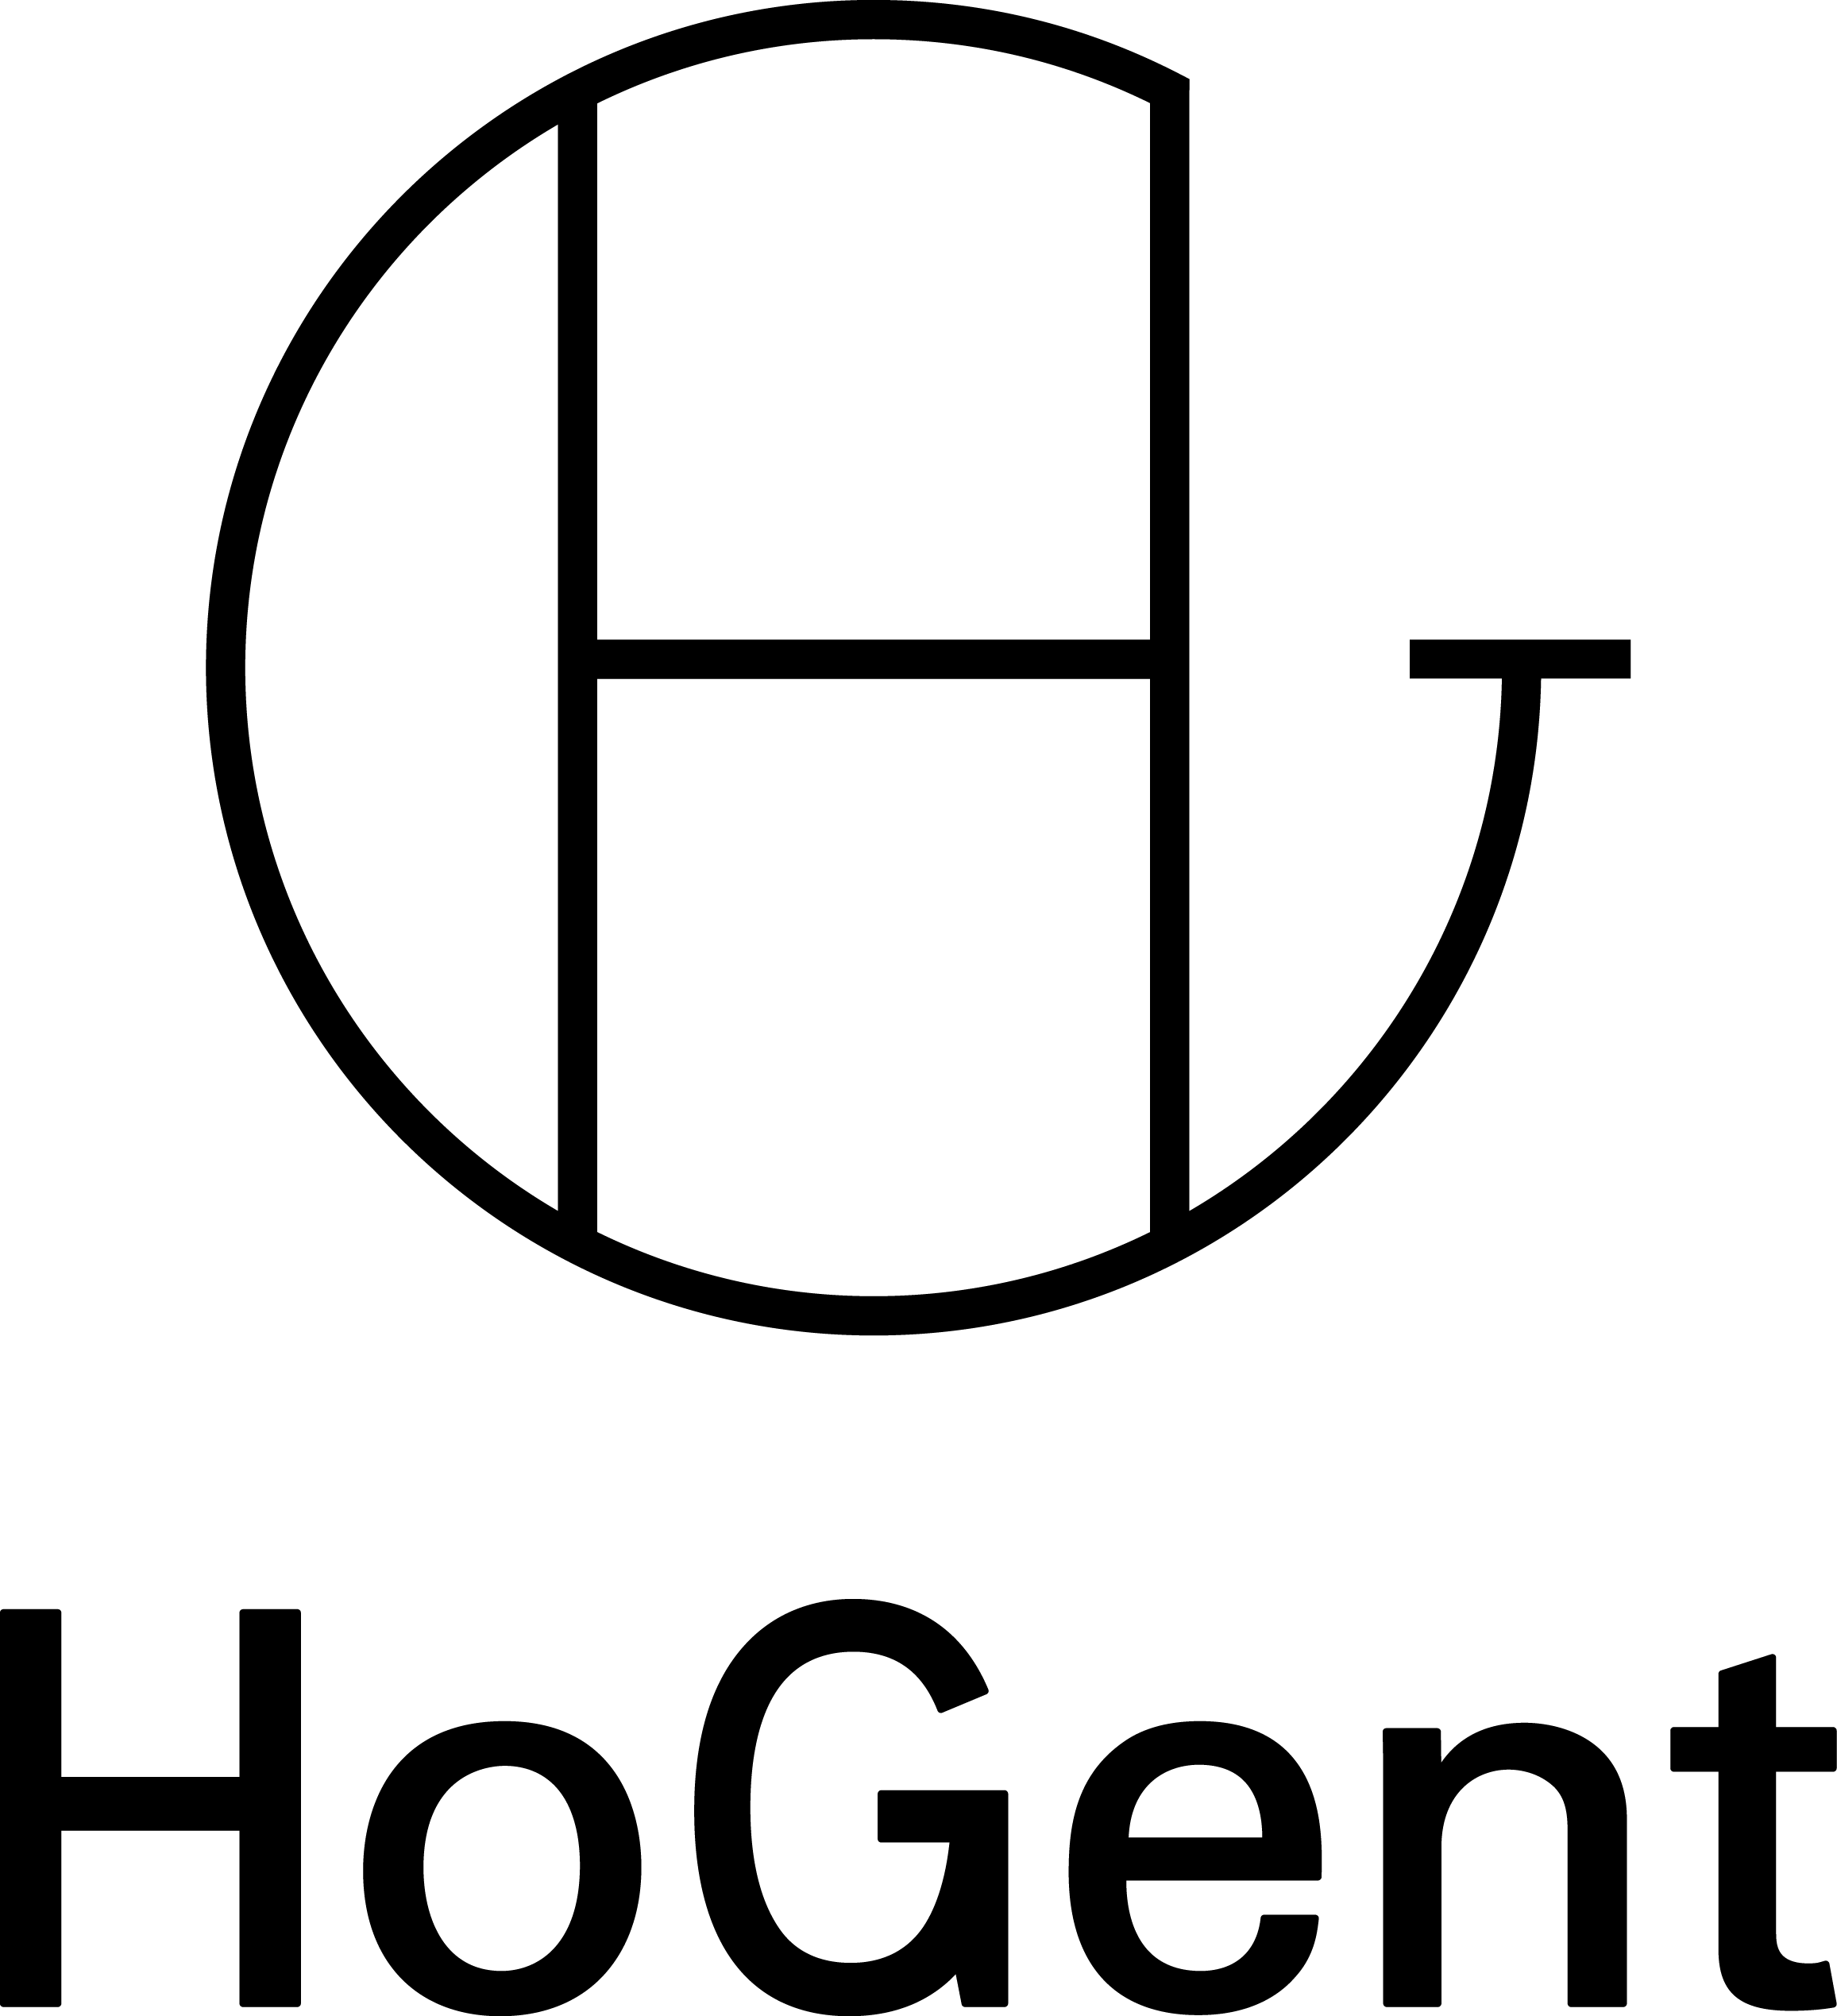
\includegraphics[width=2.5cm]{img/HG-beeldmerk-woordmerk}\\[.5cm]
    \faculteit\\[3cm]
    \titel
    \vfill
    \student\\[3.5cm]
    \rapporttype\\[2cm]
    Promotor:\\
    \promotor\\
    Co-promotor:\\
    \copromotor\\[2.5cm]
    Instelling: \instelling\\[.5cm]
    Academiejaar: \academiejaar\\[.5cm]
    \examenperiode
    \endgroup

  \end{center}
  \restoregeometry
\end{titlepage}

% Schutblad

\emptypage


\begin{titlepage}
  \newgeometry{top=5.35cm,bottom=1.5cm,left=1.5cm,right=1.5cm}
  \begin{center}

    \begingroup
    \rmfamily
    \faculteit\\[3cm]
    \titel
    \vfill
    \student\\[3.5cm]
    \rapporttype\\[2cm]
    Promotor:\\
    \promotor\\
    Co-promotor:\\
    \copromotor\\[2.5cm]
    Instelling: \instelling\\[.5cm]
    Academiejaar: \academiejaar\\[.5cm]
    \examenperiode
    \endgroup

  \end{center}
  \restoregeometry
\end{titlepage}


\begin{abstract}
% TODO: De "abstract" of samenvatting is een kernachtige (max 1 blz. voor een
% thesis) synthese van het document. In ons geval beschrijf je kort de
% probleemstelling en de context, de onderzoeksvragen, de aanpak en de
% resultaten.
Vandaag komt cybercrime meer en meer voor bij bedrijven. Professionele hackers en oplichters proberen binnen te dringen in een netwerk van een bedrijf om gevoelige informatie te verkrijgen en te gebruiken of eerder te misbruiken. In deze thesis zal worden onderzocht of de algemene best practices om een webserver met ASP.net-applicatie op te zetten, voldoende zijn om beschermd te zijn tegen enkele van de gevaarlijkste aanvallen. Daarvoor moet er eerst een webserver met ASP.net-applicatie worden opgezet in een virtueel netwerk waarop deze best practices geïmplementeerd zijn. \newline

De aanvallen worden gekozen door vooraf een risico-analyse te maken waarin per laag van het TCP/IP-model wordt gekeken naar mogelijke aanvallen. Deze aanvallen zullen worden besproken en krijgen een cijfer toegekend dat de risicofactor moet voorstellen. Bij het einde van de risico-analyse wordt er een tabel samengesteld waarbij de aanvallen met de grootste risicofactor bovenaan staan. \newline

De vier aanvallen met de grootste risicofactor zullen uitvoerig worden besproken en gesimuleerd om te kijken of de best practices die eerder geïmplementeerd zijn voldoende zijn ter berscherming. Deze aanvallen zullen worden uitgevoerd vanaf een Kali Linux-aanvallersmachine die een verbinding heeft met het netwerk. Na het uitvoeren van een aanval kan er gekeken worden of de best practices deze aanval hebben kunnen tegenhouden of dat er extra maatregelen moeten worden genomen. Indien er extra beveiliging moest worden geïmplementeerd, werden deze stappen toegevoegd aan de best practices. \newline

Na het onderzoek kon er worden geconcludeerd dat de best practices voldoende zijn voor één aanval, maar niet voldoende bescherming gaven tegen de drie andere aanvallen. Om deze reden worden de best practices aangevuld met enkele stappen om de webserver met een ASP.net-applicatie zo veel veiliger te maken.
\end{abstract}

\chapter*{Voorwoord}
\label{ch:voorwoord}
% TODO: Vergeet ook niet te bedankten wie je geholpen/gesteund/... heeft
Deze scriptie zou niet tot stand zijn gekomen zonder de hulp van mijn stagementor en co-promotor de heer Selami Top. Bij het uittesten en het onderzoeken van de onderzoeksvragen werd gebruik gemaakt van het netwerk van Hardo bvba, het bedrijf waarvan de heer Selami Top zaakvoerder is. Dit zorgde ervoor dat alle conclusies en antwoorden bedrijfsecht zijn en gaf mij een betere kijk op een realistische beveiliging. \newline

Verder wil ik ook mijn promotor de heer Bert Van Vreckem bedanken die mij enorm heeft geholpen om deze bachelorproef tot stand te brengen. Zijn structurele en inhoudelijke tips brachten deze scriptie naar een hoger niveau. Het delen van zijn kennis zorgde er ook voor dat dit onderzoek een betere kwaliteit heeft. \newline

Mijn ouders Johan Baele en Kathleen Van Wassenhove zijn ook een grote hulp geweest. Zij hebben mij enorm gesteund tijdens het onderzoeken van dit onderwerp en hebben mij geholpen bij het nalezen van de eindtekst en het verbeteren van enkele taal -en layoutfouten. \newline

Tot slot wil ik alle auteurs bedanken van de boeken, websites, handleidingen, videolessen, ... die ik heb gelezen. Deze boden mij eveneens de kans de kwaliteit van deze scriptie naar een hoger niveau te halen en mijn persoonlijke kennis en inzichten te verruimen.


\tableofcontents

% Als je een lijst van afkortingen of termen wil toevoegen, dan hoort die
% hier thuis. Gebruik bijvoorbeeld de ``glossaries'' package.

%%---------- Kern --------------------------------------------------------

\chapter{Inleiding}
\label{ch:inleiding}
"`The bad guys are winning"'. Met deze woorden uit een artikel van \cite{Wiener-Bronner2014} is het duidelijk dat vandaag de dag cybercrime meer en meer voorkomt. Professionele hackers en oplichters proberen binnen te dringen in een netwerk/server van een bedrijf om gevoelige informatie te verkijgen en te gebruiken of misbruiken om het bedrijf op te lichten. Daarom is het belangrijk om een zeer goed beveiligd netwerk te hebben tegen bedreigingen van zowel binnen als buiten het bedrijf. Dat is ook één van de doelstellingen in dit onderzoek. \newline

In deze scriptie zal een fictief netwerk worden opgezet dat een domeincontroller en een webserver zal bevatten. Deze beide virtuele machines zullen worden geconfigureerd volgens de algemene best practices om zo de beveiliging van deze servers te verbeteren. Er zijn natuurlijk honderden verschillende soorten aanvallen en mogelijkheden tot cybercrime om tot een netwerk binnen te dringen. Enkele van de meest voorkomende aanvallen zijn SQL-injectie, exploits \citep{Siddharth2006}, DDoS, port scans en social engineering \citep{Gibson2011}. Daarnaast bestaan er natuurlijk nog heel wat andere soorten.

Er moet dus ergens een keuze worden gemaakt welke aanvallen er in dit onderzoek zullen worden besproken. Dit zal gebeuren aan de hand van een risico-analyse van de webserver om te kijken welke aanvallen het meeste kans hebben om te worden uitgevoerd en dus van belang zijn. De aanvallen die de grootste kans tot slagen hebben of die het meeste schade kunnen toebrengen aan de webserver zullen dan later in dit onderzoek één voor één worden besproken. \newline 

Deze aanvallen zullen dan ook worden uitgevoerd met een Kali Linux-aanvallersmachine tegen de webserver om te kijken of de eerder geïmplementeerde best practices voldoende zijn om de server te beveiligen, of dat er extra maatregelen moeten worden getroffen. Dit heeft niet alleen als doel om de best practices aan te vullen en te verbeteren, maar ook om de typische aanpak van beveilingsproblemen, waarbij er enkel wordt gehandeld nadat er iets is gebeurd, te veranderen. Het probleem hierbij is dat er niet proactief wordt afgehandeld maar dat er eerst een aanval heeft plaatsgevonden, alvorens er naar een oplossing wordt gezocht. Dit kan resulteren in schade of diefstal binnen het netwerk. Het is dus belangrijk dat het ad-hoc controleren op fouten niet de meest gebruikte beveiligingsmanier is.


\section{Probleemstelling en onderzoeksvraag}
\label{sec:onderzoeksvragen}

% TODO: Wees zo concreet mogelijk bij het formuleren van je
% onderzoeksvra(a)g(en). Een onderzoeksvraag is trouwens iets waar nog
% niemand op dit moment een antwoord heeft (voor zover je kan nagaan).
\subsection{Zijn de best practices voor een webserver voldoende als beveiliging tegen een externe en/of interne aanval?}

Allereerst wordt de webserver geconfigureerd voglens de best practices van \cite{Cott2012}, \cite{Microsoft2013}, \cite{Poley2013}, \cite{Posey2011} en \cite{Vialle2012}. Daarna wordt er een risico-analyse uitgevoerd en wordt er gekeken naar welke aanvallen relevant zijn en welke de hoogste risicofactor hebben. De aanvallen met de hoogste risicofactor zullen worden uitgevoerd tegen de server om na te gaan of de geïmplementeerde best practices voldoende zijn om deze aanvallen af te weren. Indien dit niet het geval is dan zal er een mogelijke oplossing worden vermeld om te implementeren op de server of in het netwerk. Dit heeft als doel om de best practices aan te vullen en te optimaliseren voor een veiligere webserver.


\chapter{Methodologie}
\label{ch:methodologie}

% TODO: Hoe ben je te werk gegaan? Verdeel je onderzoek in grote fasen, en
% licht in elke fase toe welke stappen je gevolgd hebt. Verantwoord waarom je
% op deze manier te werk gegaan bent. Je moet kunnen aantonen dat je de best
% mogelijke manier toegepast hebt om een antwoord te vinden op de
% onderzoeksvraag.

Dit onderzoek bestaat uit de volgende methodiek:
\begin{enumerate}
	\item Een degelijke basiskennis is vereist, dus het verrichten van een onderzoek en het lezen van lectuur is een essentiële eerste stap.
	\item Het opzetten van een goede testomgeving met één Windows Server 2012 R2 domeincontroller, één Windows Server 2012 R2 webserver, met ASP.net-applicatie draaiende als slachtoffer, en één Kali Linux-machine als aanvaller. De Webserver zal worden geconfigureerd volgens de best practices.
	\item Een risicoanalyse uitvoeren en kijken wat de belangrijkste bedreigingen zijn voor dit type systemen.
	\item Met behulp van penetration testing tools beveiligingsproblemen zoeken en uitbuiten. Hier wordt er vanuit gegaan dat er geen fysieke toegang is tot de server. Een boot-cd insteken, rebooten en het administrator wachtwoord wijzigen zal dus niet lukken. Er wordt een lijst opgesteld met welke aanvallen er zullen worden uitgevoerd en welke hiervan succesvol werden uitgevoerd en welke hebben gefaald. Indien een aanval succesvol werd uitgevoerd, dan zullen de best practices moeten worden aangevuld.
	\item Het uitvoeren van een post-mortem om sporen van inbraak bloot te leggen en te kijken waar het probleem zich bevindt.
\end{enumerate}

\begin{figure}[H]
\begin{center}
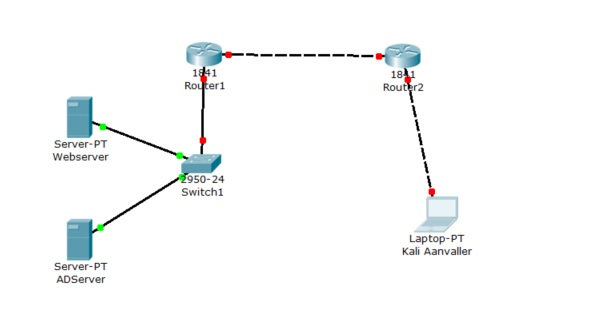
\includegraphics{img/Situatie}
\end{center}
\caption{Proefopstelling}
\label{img:situatie}
\end{figure}

In figuur~\ref{img:situatie} is te zien welke machines allemaal nodig zijn om dit onderzoek tot een goed einde te brengen. Ten eerste is er een Active Directory-server nodig die ook domeincontroller is in het domein. Deze server is tegelijkertijd ook nog DNS-server. Dan is er de webserver die lid is van hetzelfde domein als de ADServer natuurlijk. Deze zijn aangesloten aan een switch en een router. Ten slotte is er ook nog een aanvallersmachine om te proberen de server te hacken. Deze is ook aangesloten aan een router op een andere locatie. Tot slot wordt er gebruik gemaakt van VMWare Workstation om al deze virtuele machines met elkaar te verbinden.

%% TODO: de structuur en titel van deze hoofdstukken hangen af van je
% eigen onderzoek. Elke fase in je onderzoek kan een eigen hoofdstuk krijgen. Kies telkens een gepaste titel. ``Corpus'' is *GEEN* gepaste titel
\chapter{Opzetten servers met best practises beveiliging}
%Hier ga ik schrijven over wat de best practises zijn om een webserver te beveiligen en ga ik zeggen hoe je deze moet configureren/implementeren
\section{Installatie + configuratie ADServer}
De Windows Server 2012 R2-virtuele machine, genaamd \textit{ADServer}, is de eerste die moet worden opgezet. In VMWare Workstation wordt er 60GB geheugen gealloceerd voor deze virtuele machine samen met één netwerkadapter en 2GB aan RAM-geheugen. Nadat Windows Server 2012 R2 is geïnstalleerd op deze virtuele machine, krijgt deze de naam \textit{ADServer} en wordt deze heropgestart. Daarna kan er begonnen worden met het installeren van de nodige rollen. De eerste rol die wordt geïnstalleerd is de rol textit{Active Directory Domain Services}. Daarna wordt de ADServer opgewaardeerd naar domeincontroller in het fictieve domein \textit{Baele.be}. Op de server is één netwerkadapter aanwezig en deze wordt handmatig ingesteld. De server krijgt als IP-adres 192.168.1.2 mee, als subnetmask 255.255.255.0, als default gateway 192.168.1.2 en als DNS-server 127.0.0.1. \newline

Het volgende dat moet gebeuren is het installeren en configureren van de DNS-rol. Dit is vrij simpel en neemt niet veel tijd in beslag. In het scherm \textit{DNS-beheer} wordt er in het tabblad \textit{Zones voor reverse lookup}, een zone aangemaakt met de naam\textit{ 1.168.192.in-addr.arpa} en daarna wordt er een PTR-record aangemaakt dat verwijst naar de zonet geconfigureerde LANadapter met het juiste IP-adres. Hierna wordt de DHCP-rol geïnstalleerd en wordt er een nieuwe scope aangemaakt met de naam \textit{TestScope}. Het eerste IP-adres in het bereik is 192.168.1.1 en het laatste 192.168.1.254. De adressen van 192.168.1.1 tot 192.168.1.20 worden uitgesloten voor distributie. De WebServer wordt de router, dus het IP-adres dat hier wordt meegegeven is 192.168.1.3. Dit is het IP-adres dat later aan de router/WebServer wordt gegeven. \newline

\section{Installatie + configuratie WebServer}
De installatie gebeurt op dezelfde manier als bij de voorgaande machine, maar in dit geval wordt de machine \textit{WebServer} genoemd en zijn er twee netwerkadapters aanwezig, één die is verbonden met het internet (internetadapter) en een andere die is verbonden met het LAN (LANadapter). De internetadapter staat geconfigureerd als NAT en de IP -en DNS-informatie worden beiden automatisch toegewezen. Bij de LANadapter zijn de instellingen anders. Hier staat deze configureerd als \textit{Custom: specific virtual network} en wordt er gekozen om het virtuele network de naam \textit{VMnet0} mee te geven. Hierdoor moeten de IP -en DNS-instellingen handmatig worden geconfigureerd. De server krijgt al IP-adres 192.168.1.2 mee, als subnetmask 255.255.255.0, als default gateway 192.168.1.2 en als DNS-server 127.0.0.1. \newline 

Deze server wordt ook lid gemaakt van het domein \textit{Baele.be}. Verder wordt er ook de rol \textit{Externe Toegang} toegevoegd. Deze stellen we zo in dat de netwerkadapter van waar het internet komt, wordt gebruikt voor andere hosts die verbonden zijn met het netwerk en die op het internet moeten komen. De WebServer wordt dus zo een router. \newline

Op deze server is het belangrijk dat de rol \textit{Internet Information Service 8} (IIS8) is geïnstalleerd. Dit gebeurt default bij het installeren van de rol \textit{Externe Toegang}. Verder is de installatie van databanksoftware ook nodig. In dit geval wordt er gebruik gemaakt van Microsoft SQL Management Studio 2014. Bij deze installatie is het aan te raden om \textit{Use Microsoft Update to check for updates} aan te vinken. Na de installatie wordt er een testdatabase aangemaakt met de naam \textit{TestDatabase}. In deze database wordt er een tabel aangemaakt met de naam \textit{People} met de rijen \textit{PeopleID, Fname, Lname}. In deze tabel moeten twee willekeurige waarden worden gestoken. Tot slot wordt er nog een nieuwe stored procedure aangemaakt met de volgende inhoud:
\begin{verbatim}
Create Procedure Test_GetPeople
AS
Select * from People;
\end{verbatim}

De volgende stap is om een basis ASP.net-applicatie te maken en dit wordt gedaan met de hulp van \cite{Nuckolls2011}. Met behulp van deze persoon zijn tutorial, de link is te vinden in de bibliografie, is er direct een ASP.net-applicatie met een achterliggende database toegevoegd zoals te zien is in figuur~\ref{img:ASPapp}. \newline

\begin{figure}[H]
\begin{center}
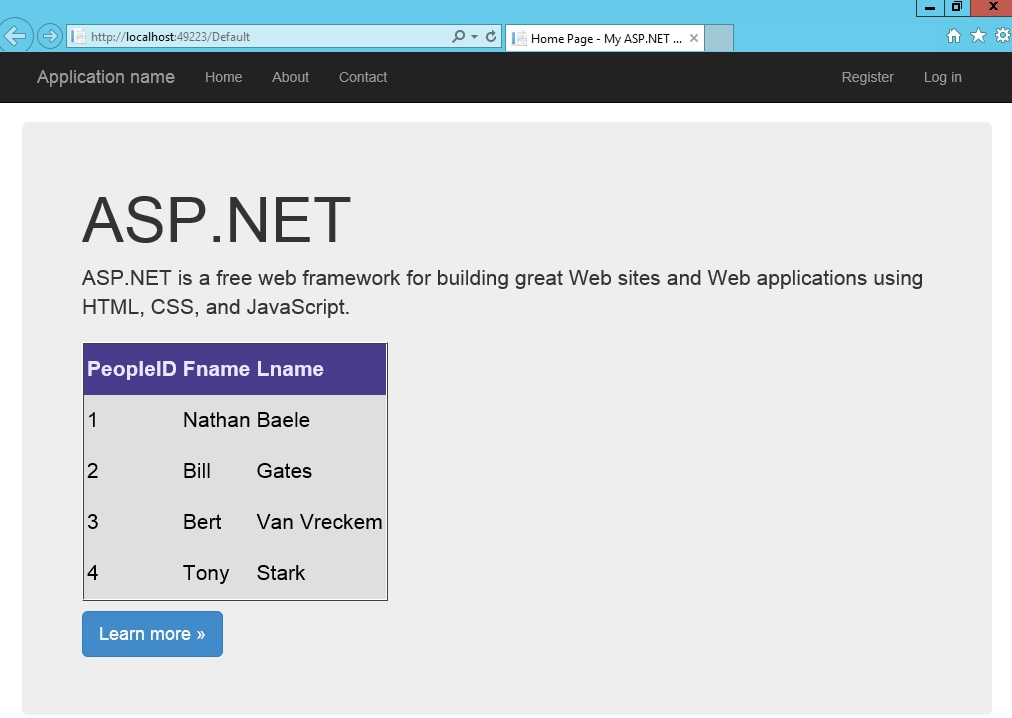
\includegraphics[scale=0.45]{img/ASPapp}
\end{center}
\caption{Voorbeeld van een basis applicatie.}
\label{img:ASPapp}
\end{figure}

\section{Installatie + configuratie aanvallersmachine}
De derde en laatste virtuele machine die nodig is in dit onderzoek is de Kali Linux-aanvallersmachine. Deze is vrij makkelijk te installeren en heeft ook niet zo hoge systeemvereisten. Voor deze machine is er maar 20Gb aan gealloceerd geheugen nodig samen met 1 netwerkadapter die op \textit{VMnet0} staat en 512MB aan RAM-geheugen. Bij het starten van de installatie moet er worden gekozen voor \textit{graphical install}. De meeste stappen zijn voor de hand liggend, maar bij partition disks wordt er het best \textit{guided-use entire disk} geselecteerd. De naam van de machine wordt ingesteld op \textit{KaliAanvaller}. Op het moment dat er wordt gevraagd van welk netwerk deze computer deel uitmaakt, wordt er \textit{baele.be} gekozen. Voor de rest zijn de overige stappen niet zo belangrijk en is de installatie zo afgerond.

\section{Besturingssysteem best practices WebServer}
Nu de webserver is geïnstalleerd, kan er worden begonnen met het toepassen van de best practices. Het is zeer belangrijk dat dit wordt gedaan alvorens de server wordt opgenomen in het netwerk. In dit deel worden alle best practices van het besturingssysteem besproken, van een sterk wachtwoordbeleid tot het regelmatig updaten van de server.

\subsection{Wachtwoordbeleid}
\subsubsection{Wachtwoord geschiedenis afdwingen}
Dit is een policy die ervoor zorgt dat gebruikers, als ze hun wachtwoord moeten wijzigen, niet tussen steeds dezelfde wachtwoorden kunnen wisselen. Er kunnen in totaal tot wel 24 wachtwoorden opgesalgen worden in de wachtwoordgeschiedenis. Zo is de kans klein dat gebruikers voortdurend wisselen tussen dezelfde wachtwoorden. Als een gebruiker slim is kan hij zijn wachtwoord gewoon 24 keer na elkaar wijzigen om dan terug zijn eerste wachtwoord te gebruiken. Dit kan ook worden voorkomen worden door een \textit{Minimum Password Age Policy} in te stellen zodat een wachtwoord bijvoorbeeld maar om de 2 dagen kan worden veranderd. \citep{Stanek2009} \newline

Dit kan worden geïmplementeerd door naar het \textit{Lokaal beveiligingsbeleid} te gaan en daar te klikken op het \textit{Wachtwoordbeleid}. Er is te zien dat de \textit{Minimale wachtwoordduur} default staat ingesteld als 1 dag en de wachtwoordgeschiedenis op 24 wachtwoorden. Deze best practices staat correct ingesteld en moet dus niet worden gewijzigd.

\subsubsection{Wachtwoord regelmatig wijzigen}
Een andere best practice is om het wachtwoord regelmatig eens te veranderen. Dit kan mondeling gebeuren, maar het meest efficiënte is om dit ook te doen aan de hand van een policy. Er kan terug worden gegaan worden naar de voorgaande locatie en daar kan er worden gekozen voor \textit{Maximale wachtwoordduur}. Deze staat default op 42 dagen . Dit is een goede waarde voor netwerken waar beveiliging zeer belangrijk is want daar wordt er meestal gekozen voor een waarde tussen de 30-90 dagen. Bij netwerken waar de beveiliging niet zo belangrijk is, kan dit eerder 120-180 dagen zijn. \citep{Stanek2009}

\subsubsection{Minimale wachtwoordlengte}
Deze policy, die ook te vinden is op dezelfde plaats als de vorige policies, zorgt ervoor dat een gebruiker zijn wachtwoord een minimale lengte moet hebben. Dit heeft als bedoeling om het brute force kraken van wachtwoorden moeilijker tot onmogelijk te maken. Default staat deze policiy op 7 dagen maar \cite{Stanek2009} raadt aan om deze policy in te stellen op een lengte van minstens 14 karakters. Dit omdat een wachtwoord van 7-8 tekens vandaag op een korte tijd wordt gekraakt door het toepassen van brute force wachtwoord kraken met moderne hardware.

\subsubsection{Complexiteit van het wachtwoord}
Het spreekt voor zich dat een wachtwoord zoals \textit{123456} niet acceptabel is. Daarom is het belangrijk dat er een policy is die de complexiteit van een wachtwoord verzekerd. Dit kan alweer gevonden worden op voorgaande locatie waar de policy \textit{Wachtwoorden moeten voldoen aan complexiteitsvereisten} kan worden ingeschakeld. Dit zorgt ervoor dat de wachtwoorden minstens 6 tekens moeten hebben, er kunnen geen gebruikersnamen of gewone namen in voorkomen en wachtwoorden moeten minstens 3 van de 4 verschillende soorten karaktertypes bevatten (normale letters, hoofdletters, nummers en symbolen). \citep{Stanek2009}

\subsection{Accountbeheer}
\subsubsection{Uitschakelen van Administrator-account}
Wat allereerst moet gebeuren, is het uitschakelen van de inlognaam \textit{Administrator}. Dit omdat elke persoon weet dat het default account een specifieke naam heeft. Het is voor hackers op deze manier gemakkelijker om binnen te breken . Dit account kan uitgeschakeld worden door op de ADServer naar de \textit{Active Directory - gebruikers en computers} te gaan en daar bij \textit{Users} te rechterklikken op het account \textit{Administrator} en deze dan uit te schakelen.

\subsubsection{Aanmaken eigen administrator-account}
Nadat in de vorige stap het default administrator-account is uitgeschakeld, moet er natuurlijk weer een nieuw account komen zodat er toch nog administrator-taken kunnen worden uitgevoerd. Dit kan gedaan worden door op dezelfde locatie als bij de voorgaande stap een nieuwe gebruiker toe te voegen, in dit geval met de naam \textit{BaeleAdministrator}, en deze lid te maken van de groepen \textit{Administrators, Domeinadministrators en domeincontrollers}. Nu is het best om eerst uit te loggen en daarna opnieuw terug in te loggen met het nieuwe account.

\subsection{Updates}
Nog een belangrijk onderdeel van een server met best practice beveiliging, is het regelmatig downloaden en installeren van updates. Bij het ontdekken van een nieuw zwak punt of exploit in de software, wordt dit al binnen enkele uren op het internet geplaatst en wordt er onmiddelijk gezocht naar een oplossing. Als de server en de applicaties continue worden geupdate, dan is de kans veel kleiner dat er een exploit zal worden uitgebuit. \citep{Cott2012}. Automatische updates worden echter zo goed als nooit gedaan. De voorgestelde updates worden best eerst door de administrator gedownload en uitgetest in een virtuele testomgeving zodat er zekerheid is dat deze update geen problemen met zich meebrengt. Na een geslaagde test, kan de update op de webserver worden geïnstalleerd.

\subsection{Backup}
Het maken van geautomatiseerde backups is essentieel voor een server binnen een netwerk. Een fout, een probleem of een aanval kan op elk moment van de dag voorkomen. Als dit gebeurt, moet het mogelijk zijn om het systeem terug te zetten door een eerder gemaakte backup. In de Windows Server Backup-wizard kan dit worden ingesteld voor elke harde schijf. In dit geval wordt er enkel elke nacht om 03:00u een back-up genomen van de C-schijf, maar dit varieert van bedrijf tot bedrijf en hangt af van hoeveel geheugen er beschikbaar is voor back-ups en welke dataschijven het belangrijkste zijn. 

\subsection{Firewall}
De firewall is enorm belangrijk en heeft een standaard configuratie. Er is echter één aanpassing van de configuratie die in de praktijk veel wordt toegepast en die ook door \cite{Nabors2013} wordt genoemd als een best practise-instelling voor een Firewall-configuratie. Dit betreft het blokkeren van alle uitgaande verbindingen die niet overeenkomen met één van de gedefinieerde regels. \newline 

Dit wordt verkregen door naar de \textit{eigenschappen} te gaan en daar in alledrie de profielen de uitgaande verbindingen op "`blokkeren"' te zetten. Standaard staat dit geconfigureerd als \textit{toestaan}. Hierna kunnen er eigen inkomende en uitgaande regels geconfigureerd worden naargelang de applicaties die op de server komen te staan en afhankelijk van welke poorten open of dicht moeten zijn. Bij uitgaande verbindingen is het belangrijk dat de TCP-poorten 80 (hhtp) en 443 (https) worden toegevoegd aan de uitzonderingen. Nadat deze poorten zijn toegevoegd ziet de verzameling van toegestane uitgaande verbindingen eruit als in figuur~\ref{img:FirewallUitgaand}.

\begin{figure}[H]
\begin{center}
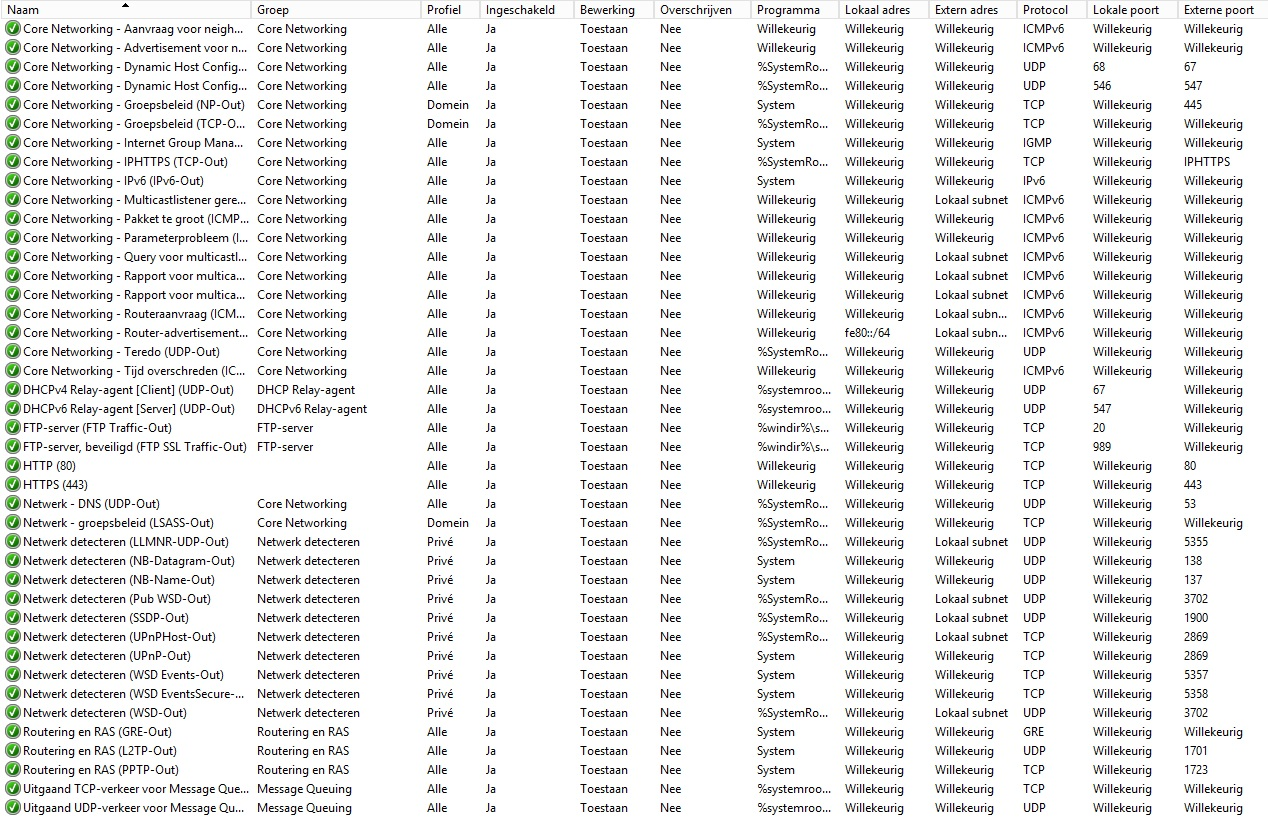
\includegraphics[scale=0.45]{img/FirewallUitgaand}
\end{center}
\caption{Alle toegestane uitgaande verbindingen}
\label{img:FirewallUitgaand}
\end{figure}

\subsection{Anti-virus}
\subsubsection{Goede anti-virus installeren}
Een degelijke anti-virus is enorm belangrijk om een server, computer of ander online apparaat te beschermen. Bij het gebruiken van een desktop of laptop voor persoonlijk gebruik, is een gratis versie van een bepaalde anti-virus-software voldoende. In een bedrijfsomgeving is het beter dat er een betaalde versie wordt gekozen daar deze veel meer functies en opties hebben. Microsoft heeft een gratis beveiligingssoftwarepakket genaamd \textit{Microsoft Security Essentials}, maar deze heeft geen versie die op de Windows Server 2012-besturingssystemen kan worden geïnstalleerd. Er is gelukkig wel een manier om de Windows 7-versie van deze software te installeren.

Men surft eerst naar de website van Microsoft Security Essentials om daar de recentste versie te downloaden en dit voor een Windows 7 64-bit machine. Als deze installer is gedownload dan moet er gegaan worden naar de eigenschappen om daar de compatibiliteit te veranderen naar Windows 7. Hierna moet er een opdrachtprompt gestart worden en moet er genavigeerd worden naar de map waar de installer is in geplaatst. Daar wordt met het onderstaand script:
\begin{verbatim} mseinstall /disableoslimit \end{verbatim} 
de installer succesvol gestart. Bij de installatie hoeft er enkel op \textit{volgende}  te worden gedrukt en de software wordt succesvol geïnstalleerd. Hierna kan er een eerste scan worden gestart die de hele server onderzoekt op virussen en spyware nadat deze zichzelf heeft bijgewerkt met de nieuwste updates. \citep{Herring2014}

\begin{figure}[H]
\begin{center}
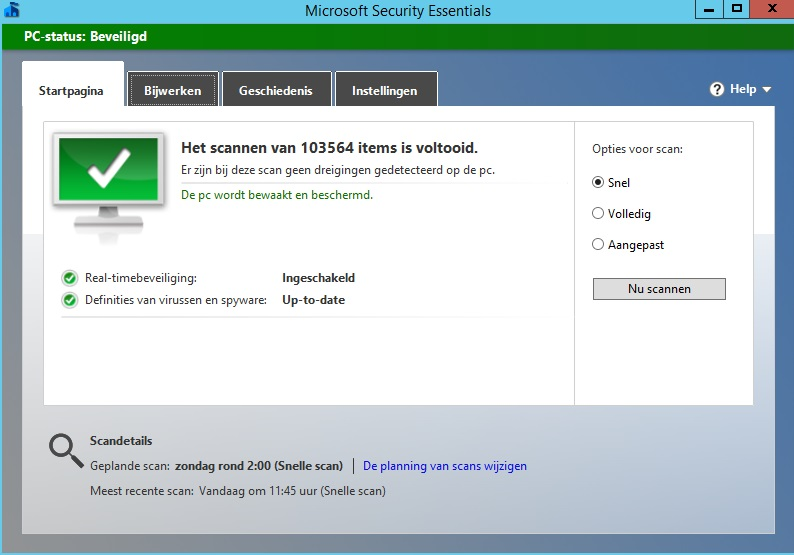
\includegraphics[scale=0.60]{img/AntiVirus}
\end{center}
\caption{Voorbeeld van succesvolle scan met volgende geplande scan}
\label{img:AntiVirus}
\end{figure}

\subsubsection{Regelmatig scannen en updaten}
Het spreekt voor zich dat deze anti-virus regelmatig moet worden ge-update zodat wanneer er een nieuwe bedreiging wordt gesignaleerd, deze direct kan worden toegevoegd  aan de anti-virus software. Door het dagelijks uitvoeren van updates en een anti-virusscan blijft de server optimaal beschermt. Het beste is om dit 's nachts te doen als het netwerk niet wordt gebruikt. Dit omde gebruikers van het netwerk tijdens de werkuren niet te belasten. 

\section{IIS best practices WebServer}
\subsection{Dedicated server}
Het is volgens \cite{Microsoft2013} gebruikelijk om de webserver en de domeincontroller van elkaar te scheiden. Dit heeft als reden dat er geen lokale accounts zijn op een domeincontroller. Deze lokale accounts zijn belangrijk voor een veilige IIS-server. Het samenplaatsen van een DC en een webserver beperkt de beveiligingsmogelijkeden enorm. Bijvoorbeeld een nieuwe exploit die door een hacker wordt gebruikt zal zo niet alleen de webserver aantasten, maar ook het hele netwerk. Daarom worden de DC en de webserver dus het best gescheiden, zoals in deze opstelling het geval is.

\subsection{Inetpub}
De inetpub-map wordt bij elke installatie van IIS aangemaakt en standaard geplaatst op de C-schijf. Aangezien dit dezelfde schijf is waarop het besturingssysteem staat, is het gebruikelijk om deze map op een aparte schijf te zetten zodat de toegang tot deze schijf beter kan beschermd worden. De schijf waar het besturingssysteem opstaat, kan nooit zo goed worden beschermd alsop een aparte schijf. \citep{Darmanin2014}

\subsection{Modules}
In totaal bevat IIS meer dan 30 modules. Deze moeten niet allemaal actief zijn. In de IIS manager kunnen er in het modulescherm van de geselecteerde website bepaalde modules op inactief worden gezet. Er moet een lijst worden opgemaakt van welke modules nodig zijn en welke overbodig zijn. De overbodige modules kunnen dan worden uitgeschakeld door deze uit de lijst te verwijderen. In onderstaand voorbeeld blijven alle modules staan want deze zijn nodig voor het uitvoeren van de applicatie. \citep{Darmanin2014} \citep{Microsoft2013}

\begin{figure}[H]
\begin{center}
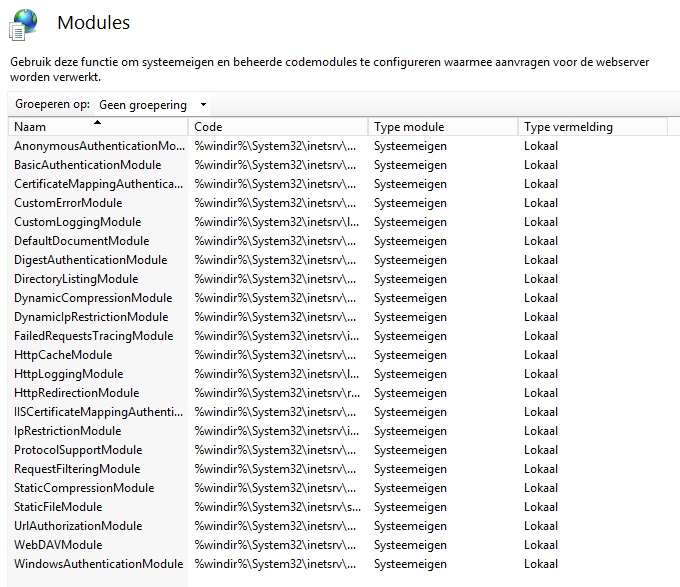
\includegraphics[scale=0.60]{img/IIS_Modules}
\end{center}
\caption{Alle modules die geactiveerd blijven}
\label{img:IISModules}
\end{figure}

\subsection{Opties methode uitschakelen}
De opties \textit{methode} geeft een lijst van methodes weer die worden ondersteund door de webserver. Dit kan waardevolle informatie opleveren voor een hacker. Het is dan ook een best practice om deze methode uit te schakelen. Dit gebeurt door het woord \textit{OPTIONS} uit te sluiten van de \textit{HTTP Verb request filtering rules} in IIS. Dit wordt verkregen door de website te selecteren in de IIS-manager en dan te dubbel klikken op \textit{aanvraagfiltering} en naar het tabblad \textit{HTTP-termen} te gaan. Hier wordt als actie gekozen \textit{Term weigeren...} en wordt \textit{OPTIONS} ingevuld en op OK gedrukt. Nu staat deze regel als enige in de lijst en is deze best practice aangepast zoals in figuur~\ref{img:IISOptions} te zien is. \citep{Darmanin2014}

\begin{figure}[H]
\begin{center}
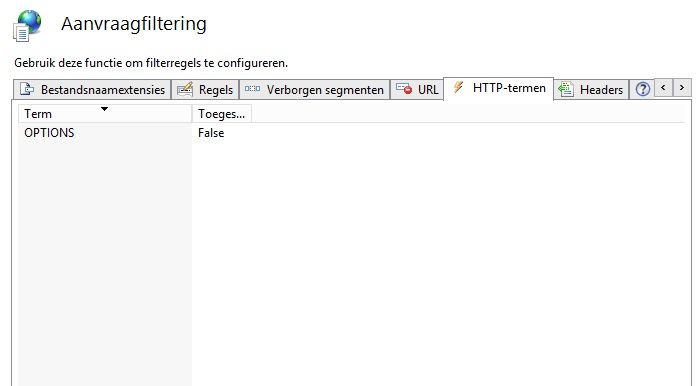
\includegraphics[scale=0.60]{img/IIS_Options}
\end{center}
\caption{De term OPTIONS wordt niet toegestaan}
\label{img:IISOptions}
\end{figure}

\subsection{Dynamische IP restricties}
Het inschakelen van de dynamic IP restrictions module zorgt ervoor dat IP-adressen, die een bepaald aantal requests hebben verzonden, worden geblokkeerd. Hierdoor worden \textit{Denial of Service-aanvallen} voorkomen. Deze module inspecteert het IP-adres van elke request en zal deze requests filteren om de IP-adressen met slechte intenties tijdelijk te blokkeren. Men doet dit door naar de IIS-manager te gaan en de naam van de website te selecteren en te dubbelklikken op \textit{beperkingen voor IP-adressen en domeinen}. In het actie paneel wordt er geklikt op \textit{instellingen voor dynamische beperking bewerken.. }en kunnen er restricties worden ingevoerd. De eerste twee vakjes moeten worden aangevinkt en de waarden kunnen naar keuze worden ingevuld, in dit geval is 5-20-200 ingevuld. \citep{Darmanin2014}

\begin{figure}[H]
\begin{center}
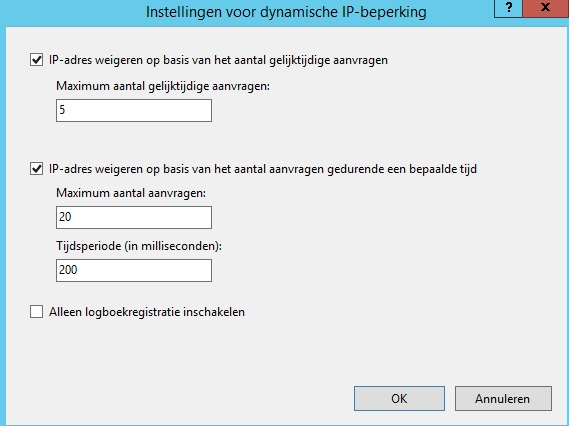
\includegraphics[scale=0.60]{img/IIS_Restrictie}
\end{center}
\label{img:IISRestrictie}
\caption{Instellingen voor dynamische IP-beperking}
\end{figure}

\subsection{Request Filtering Rules}
Het is altijd aan te raden om de verschillende types van HTTP-request die worden verwerkt door IIS te beperken. Door het instellen van uitsluitingen en regels kunnen potentieel gevaarlijke requests er nooit doorkomen. Dit gebeurt in de IIS Manager waar de juiste website wordt gekozen en waarna er wordt gedubbelklikt op \textit{Requestfilters}. Hier gaat men naar het tabblad \textit{regels} en kunnen verschillende filterregels worden toegevoegd.\citep{Darmanin2014} \citep{Microsoft2013}

\subsection{Inschakkelen logs}
Door het inschakelen van het IIS logsysteem worden verschillende HTTP-requests gelogged. Indien er zich problemen voordoen kan er hier worden gekeken om een betere kennis te vergaren over het probleem. Dit kan vrij snel en simpel worden ingeschakeld door te gaan naar de IIS manager en daar de gewenste website te selecteren en op \textit{logging} te klikken. Er wordt hier best gekozen om een nieuw bestand aan te maken daar deze bestanden vrij snel groeien. \citep{Darmanin2014} \citep{Microsoft2013}

\section{SQL Server best practices WebServer}
\subsection{Uitschakelen van onnodige features}
Nadat de software is geïnstalleerd gaat men best naar de \textit{SQL Server Configuration Manager Tool} om alle onnodige features te verwijderen. In dit geval zijn er geen extra features geïnstalleerd die niet gebruikt zijn en is dit dus overbodig. \citep{Mam2013}

\subsection{Patchen en updaten}
Zoals elk Microsoft-product wordt ook een SQL Server regelmatig voorzien van de nieuwste updates en patches om de applicatie zo goed mogelijk te beveiligen tegen hedendaagse aanvallen. Het is best dat deze updates eerst worden gedownload en geïnstalleerd in een testomgeving om daarna ze pas in de echte omgeving te implementeren. Dit kan voorkomen dat bugs in de patch de server in gevaar brengen. \citep{Mam2013}

\subsection{Loggen van aanmeldpogingen}
Het kan zeer handig zijn om logbestanden bij te houden van iedereen die zich aanmeldt op de SQL Server. Zowel de geslaagde als de mislukte login-pogingen zouden moeten worden geregistreerd. Dit kan gedaan worden door naar \textit{SQL Server Management Studio} te gaan en te rechterklikken op de gewenste SQL Server en dan \textit{eigenschappen} te selecteren. Aan de linkerkant is er de mogelijkheid om op \textit{Security} te klikken en daar kan er gekozen worden voor \textit{Both failed and successful logins}. Als dit is gebeurd, hoeft SQL enkel opnieuw worden opgestart. Vanaf nu zal dit altijd automatisch gebeuren. \citep{Mam2013}

\chapter{Risico-analyse}
Het uitvoeren van een risico-analyse kan in verschillende stappen worden onderverdeeld. Allereerst moet er een opsomming zijn van alle \textit{assets} die zullen worden onderzocht in de risico-analyse. Dan kan er gebrainstormd worden om te kijken welke soort bedreigingen er voor de specifieke server bestaan, in dit geval een webserver. Tot slot wordt er met behulp van enkele tools en wat opzoekwerk gekeken naar welk van deze bedreigingen het belangrijkste zijn. Dit wil zeggen dat er wordt gekeken naar de kans dat deze bedreiging zal plaatshebben en de mogelijke schade die deze kan toebrengen. Op deze manier worden de bedreigingen gecatalogiseerd naarmate van belangrijkheid.

\section{Assets}
In dit onderzoek wordt er gewerkt met een webserver waarop de recenste versie van Windows Server 2012 R2 staat geïnstalleerd met de volgende rollen/programma's/besturingssystemen op:
\begin{itemize}
	\item Windows Server 2012 R2 
	\item Internet Information Services 8 
	\item Externe toegang, routering 
	\item Microsoft SQL Server Express 2014 
\end{itemize}
De waarde die aan deze assets wordt meegegeven, wordt verklaard in het volgende deel.

\section{Bedreigingen en risicofactoren}
De soorten bedreigingen kunnen worden ingedeeld per laag van het TCP/IP-model. Hierdoor kan er structureel worden gekeken naar elke laag om te kijken welke bedreigingen er aanwezig zijn alvorens er wordt verder gekeken. Deze werkwijze zorgt er ook voor dat er minder snel een bedreiging over het hoofd wordt gezien. Er wordt ook gekeken naar wat de mogelijkheidsgraad is dat deze aanvallen op een webserver zullen plaatsvinden en wat de mogelijke schade kan zijn. Zo wordt er een cijfer meegegeven aan een aanval om te kijken hoe belangrijk deze is. Hoe hoger cijfer, hoe belangrijker het is om de server te beschermen tegen deze aanval. Het berekenen van dit cijfer gebeurt door deze formule: "`schade van de aanval x kans op een aanval"'. Beide factoren krijgen een cijfer van 1 tot 10 mee waar 10 de hoogste factor (meeste schade of grootste kans op een aanval) voorstelt en 1 dus het omgekeerde. \citep{Sim2005}

\subsection{Applicatielaag}
Dit is de 4de en de hoogste laag van het TCP/IP-model en is een samenvoeging van de applicatie -, presentatie -en sessielaag van het OSI-model. Deze laag bevat al de ''high-level'' protocollen zoals DNS, HTTP, Telnet, SSH, FTP, TFTP, SNMP, ... en noem maar op. Deze laag heeft ook een rechtstreekse verbinding met de eindgebruiker en de applicaties. \citep{Thomas2013}

\subsubsection{Laag 7 DoS-aanvallen}
Een DoS-aanval (of Denial of Service-aanval) die zich afspeelt in de applicatielaag kan een hele server doen crashen. Dit kan worden gedaan door één gebruiker. Indien er meerdere personen samenwerken om een netwerk/server plat te leggen dan wordt er gesproken van een DDoS-aanval (of Distributed Denial of Service-aanval). Een voordeel van DDoS-aanvallen is dat deze moeilijker zijn om na te trekken aangezien er verschillende mensen op hetzelfde moment aanvallen in plaats van één persoon bij een DoS-aanval. \citep{Blagov2014} Er zijn verschillende soorten applicatielaag DoS-aanvallen zoals RUDY (R-U-Dead-Yet) waar IIS 8 het slachtoffer wordt en XerXes waar de server via een TCP-connectie het slachtoffer wordt. \newline

De kans dat deze soort aanvallen zullen worden uitgevoerd is zeer groot aangezien het hier gaat over een webserver. Webserver zijn een gemakkelijk doelwit voor zulke aanvallen. De factor \textit{kans op een aanval} krijgt dus een 9 mee. De schade die een DoS-aanval kan veroorzaken is niet mis.  Deze kan een server of webapplicatie helemaal offline halen zolang de aanval duurt. Het spreekt voor zich dat dit vrij vervelend is, maar er is geen mogelijkheid tot diefstal van gegevens zoals kredietkaartgegevens of inloggegevens en er kan niets op de server of webapplicatie zelf worden veranderd dus de factor \textit{schade van de aanval} krijgt een 6 mee. Als hierop de formule wordt toegepast dan krijgt deze aanval een waarde van \textbf{54} mee.

\subsubsection{DNS Poisoning}
Dit is een aanval die de cache van DNS ''vergiftigd'' door valse invoer te geven. Zo kan een aanvaller een willekeurige website als facebook of google laten verwijzen naar een IP-adres van zijn eigen website met malware om zo de gebruiker op te lichten. Als een hacker toegang verkrijgt tot een DNS-server en deze valse invoeren plaatst, kan elke persoon binnen een netwerk door het surfen naar een bepaalde website bij een verkeerde website terechtkomen of zelfs bij de machine van de aanvaller zonder dat deze persoon er zelf weet van heeft. Een hacker kan toegang verkrijgen tot een DNS-server door bijvoorbeeld foutjes uit te buiten die in de DNS-software zitten. \citep{Hoffm2015} \newline

Op een webserver is de kans dat dit soort aanvallen voorkomen immens klein omdat in de meeste gevallen een DNS-server en een Webserver gescheiden zullen zijn. Zoals eerder besproken is het een best practice om de domeincontroller en de webserver op aparte machines te plaatsen en DNS zit in het merendeel van de gevallen bij de domeincontroller. Hierdoor is krijgt de factor \textit{kans op een aanval} een 1 mee. De schade die deze aanval kan veroorzaken is echter zeer groot. Als een hacker het inlogportaal van een bank namaakt en de gebruiker hier via DNS poisining naartoe stuurt, kunnen zo bankgegevens gestolen worden en dit kan grote gevolgen hebben. Hierdoor krijgt deze aanval als factor \textit{schade van de aanval} een 9 mee. Dit brengt de totale waarde van de aanval naar de waarde \textbf{9}.

\subsubsection{SQL-injectie}
Een SQL-injectie is simpel uitgelegd een aanval die slechte code in een webapplicatie gebruikt om hackers SQL-commando's in te geven in een veld om zo toegang te verkrijgen tot een database. Zo kan een hacker bijvoorbeeld bepaalde SQL-commando's ingeven in het login formulier om zo persoonlijke gegevens van anderen te verkrijgen van in de database van de webapplicatie. Bij een succesvolle SQL-injectie kan een hacker niet alleen kijken naar gegevens in een database, hij kan deze gegevens zelfs verwijderen. Dit kan gebeuren bij elk invoerveld waar de gebruiker data moet invoeren om dan data terug te ontvangen. Als deze invoer niet gevalideerd wordt, dan is de kans reeël dat wanneer bijvoorbeeld het commando \begin{verbatim} SELECT * FROM USERS; DROP TABLE USERS;\end{verbatim} wordt ingegeven, dit ook effectief wordt uitgevoerd met alle gevolgen nadien. \citep{Acunetix2014} \newline

Volgens \cite{Acunetix2014} is een SQL-injectie één van de meest voorkomende aanvallen op de applicatielaag die vandaag voorkomen. Hierdoor is de kans dus vrij groot dat een webserver met een achterliggende webapplicatie hiermee te maken krijgt. Dus de factor \textit{kans op een aanval} krijgt hier ook een 10 mee. De schade die deze aanval kan veroorzaken is natuurlijk ook zeer groot. Een goed gecoördineerde SQL-injectie kan de inloggegevens van alle gebruikers stelen en kan zelfs velden van de database verwijderen. Hierdoor krijgt de factor \textit{schade van de aanval} een 9 mee. Dit brengt de totale waarde van de aanval op \textbf{90}, hetgeen zeer hoog is.

\subsubsection{Dictionary attack telnet}
In deze aanval wordt er gekeken via een port scan of poort 23 (telnet) open is bij een specifieke machine. Indien deze poort open is dat kan er via een \textit{dictionary attack} een juiste wachtwoord/gebruikersnaam-combinate gezocht worden om via poort 23 binnen te breken in een machine. Als dit gelukt is kan er via \textit{Putty} een verbinding worden gemaakt met de doelmachine. De tool die hier het best voor wordt gebruikt is \textit{Hydra}. Deze tool staat ook in elke Kali Linux-machine bij de top 10 meest gebruikte tools. \citep{Wilde2013} \newline

Dit is een aanval die niet moeilijk aan te leren is maar die wel veel tijd en oefening vergt en hierdoor neemt de kans op een aanval toch een beetje af. Toch krijgt deze aanval nog bij de factor \textit{kans op aanval} een 7 mee. De schade die deze aanval kan aanrichten is immens. Bij een succesvolle aanval zal de hacker volledige controle krijgen over het doelwit, in dit geval een webserver. Hij kon zo alle gegevens inkijken, kopiëren en verwijderen. Zo kan er gevoelige en geheime informatie doorgespeeld worden en kunnen er allerlei soorten chantage en spionage plaatsvinden. Bij de volledige controle over een machine zijn er veel zaken die een hacker kan doen dus hierdoor krijgt de factor \textit{schade van de aanval} een 10 mee. Hierdoor komt de totale waarde van deze aanval op een \textbf{70} te staan.

\subsection{Transportlaag}
Dit is de derde laag van het TCP/IP-model en is hetzelfde als de 4de laag van het OSI-model. Deze laag is vooral gekenmerkt door de twee transportprotocollen TCP en UDP die hier op werken. De bedoeling van deze laag is om foutvrije berichten te verzenden tussen hosts. \citep{Thomas2013}

\subsubsection{Port scanning}
Een port scan kan gebruikt worden als een aanval, maar kan ook gebruikt worden voor de administrator te helpen. Bij een port scan wordt er gekeken bij een computer of een netwerk welke TCP -en/of UDP-poorten er allemaal open zijn en luisteren. Als aanvaller kan er zo gekeken worden waardat er mogelijkheden zijn om in te breken en als administrator kan er gekeken worden naar de zwakke plekken in het netwerk of op een computer/server. Via een port scan kan een administrator ook zien of er \textit{bad ports} open zijn. Dit zijn poorten die open staan omdat er een trojan horse, DDoS-tool of een andere soort van kwaadaardige software op het systeem staat. Zo kan er ook tijdig ingegrepen worden. \citep{Kessler2001} \newline

Aangezien een webserver vanaf het openbare web bereikbaar is, is er een groot risico op port scans. Er bestaan zelfs bots die automatisch port scans uitvoeren bij willekeurige websites en alle zwaktes doorgeven aan de eigenaar. Hierdoor is de factor \textit{kans op aanval} een 9. De schade daarentegen is zeer laag want een port scan zelf brengt geen schade toe tot een netwerk en is zelfs niet illegaal. Het uitbuiten van de exploits die deze port scan blootlegt, dat is wel illegaal. Het enigste wat een port scan doet is kijken door het raam van het huis, hetgeen niet strafbaar is. Pas wanneer er wordt ingebroken dan pas is het strafbaar en kan er schade zijn. Hierdoor is de factor \textit{schade van de aanval} toch een 2 aangezien het potentiële zwaktes tentoonstelt. Dit brengt de totale waarde van deze aanval op \textbf{18}.

\subsubsection{TCP SYN flood} 
Deze aanval is een soort van DOS-aanval waar de aanvaller de bekende \textit{three-way handshake} misbruikt. Bij een normale three-way handshake wordt er een SYN-bericht gestuurd naar de server met de vraag om een connectie te verkrijgen. Daarna krijgt de gebruiker een SYN-ACK terug waarme zijn request wordt geaccepteerd. Tot slot antwoordt de gebruiker met een ACK waarme de verbinding tot stand wordt gebracht (zoals te zien is in figuur~\ref{img:ThreeWayHandshake}). Bij een TCP SYN flood-aanval worden er meerdere SYN-berichten verzonden en worden er meerdere SYN-ACK berichten terug gestuurd naar de gebruiker maar deze stuurt geen enkele keer een ACK-bericht terug. Hierdoor blijven er half open verbindingen openstaan op een server en wordt er geheugen gebruikt op de server. Een voorbeeld van deze aanval is \textit{Sockstress}. \citep{Rouse2014}    

\begin{figure}[H]
\begin{center}
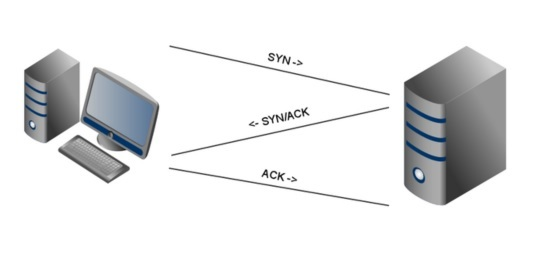
\includegraphics{img/ThreeWayHandshake}
\end{center}
\label{img:ThreeWayHandshake}
\captionsource{ThreeWayHandshake}{http://blogs.ixiacom.com/ixia-blog/tcp-portals-the-handshakes-a-lie/}
\end{figure}

Dit is een aanval die veel kan voorkomen en die ook door gerespecteerd lid van de security community \cite{Bown2013} als zeer gevaarlijk wordt beschouwd. Het feit dat de webserver rechtreeks in verbinding staat met het internet, wilt zeggen dat de kans zeer groot is dat deze aanval zal plaatsvinden dus daarom is de factor \textit{kans op aanval} een 9. Een succesvolle aanval kan een server doen vastlopen en ook al wordt de aanval gestopt, de server kan alleen maar terug werken nadat deze handmatig opnieuw is opgestart. Dit zorgt ervoor dat de webserver onbereikbaar is tot dat er iemand naar de locatie gaat en op de shutdown-knop drukt en de server weer laat rebooten. Deze aanval kan geen gevoelige gegevens wissen of stelen, maar kan wel voor een lange downtime zorgen van een website/server. Daarom krijgt deze aanval een 7 mee bij de factor \textit{schade van de aanval}. Hierdoor komt de waarde van deze aanval op \textbf{63} te staan.

\subsection{Internetlaag}
De internetlaag is de tweede laag van het TCP/IP-model en staat gelijk aan de 3de laag, de netwerklaag, in het OSI-model. Deze laag steekt de data in pakketten genaamd IP-datagrammen waar de bron -en eindbestemming van het pakket in verwerkt zitten. Deze laag is ook verantwoordelijk voor het routeren van deze pakketten. De protocollen die vooral worden gebruikt op deze laag zijn IP, ICMP en ARP. \citep{Thomas2013}

\subsubsection{Ping flood}
Een Ping flood is eigenlijk de oudste en meest primitieve vorm van een DOS-aanval want iedereen kan het doen en het is extreem gemakkelijk. Als een server een Ping flood-aanval te verduren krijgt, dan krijgt deze server zoveel ping requests dat deze het niet meer aankan omdat er teveel CPU-resources gebruikt worden. De aanvaller stuurt dan pings, via ICMP-pakketten, zonder te wachten op een antwoord. Hierdoor kan de server niet tijdig antwoorden en worden echte requests ook geblokkeerd. Dit kan leiden tot een immens vertraagde server en/of website. \citep{Grid2010}

Bij een webserver hebben deze soort aanvallen een grote kans om uitgevoerd te worden door de verbinding die deze server heeft met het internet en omdat het zo gemakkelijk is om uit te voeren. Om een soortgelijke aanval te doen heeft een persoon weinig kennis nodig, dit maakt deze aanval zo angstaanjagend omdat iedereen het zou kunnen na een tutorial van 5 minuten. Hierdoor krijgt de factor \textit{kans op aanval} een 10. De schade die deze aanval kan veroorzaken is echter vrij bescheiden. Het is niet dat een soortgelijke aanval een server kan plat gooien, maar het kan wel voor de nodige vertraging zorgen. Dit kan ervoor zorgen dat de website of server veel trager zal reageren op requests en dat de netwerkverbinding veel trager zal gaan. Aangezien deze aanval geen permanente schade kan veroorzaken maar enkel overlast, krijgt deze bij de factor \textit{schade van de aanval} een 3 mee. Hiermee komt de totale waarde van de aanval op \textbf{30}.

\subsubsection{ARP spoofing - Man in the middle}
Deze aanval wordt ook wel eens \textit{ARP cache poisoning} of \textit{ARP poison routing} genoemd. Dit is een aanval waar een aanval valse Address Resolution Protocol-berichten (ARP) over een LAN verzendt. Dit heeft als resultaat dat het MAC-adres van de aanvaller wordt gelinkt met een IP-adres van een echte computer in het netwerk. Vanaf deze link is geslaagd, zal de aanvaller alle data ontvangen die is bedoeld voor de computer waarvan de aanvaller het IP-adres gebruikt. De Man in the middle-aanval is de variant van ARP spoofing waar het verkeer tussen twee hosts eerst naar de hacker zijn machine wordt verzonden en nadat deze persoon de pakketten heeft kunnen bekijken (sniffen), dan wordt het verkeer naar de normale bestemming verzonden. Dit gebeurd zonder dat iemand er weet van heeft. Deze aanval kan alleen gebruikt worden, maar wordt in vele gevallen ook gebruikt in combinatie met een andere aanval. Bij een DoS-aanval kan ARP spoofing worden gebruikt om meerdere IP-adressen te linken aan één MAC-adres en zo het verkeer van al deze IP-adressen naar het doelsysteem waar het MAC-adres van is gebruikt. Zo wordt het doel overspoeld met verkeer. \citep{Glynn2014} \newline

Een soortgelijke aanval kan voorkomen op een webserver omdat deze rechtstreeks in verbinding staat met de router, maar deze is echter niet zo makkelijk uit te voeren als een ping flood. Hierdoor krijgt deze aanval bij de factor \textit{kans op aanval} een 8. De schade die een hacker kan toebrengen aan een server of netwerk is dan weer vrij groot. Zo kan deze alle pakketten die worden verstuurd naar een ''vergiftigde'' host om zo gevoelige informatie te verkrijgen. Als een hacker de verbinding tussen bijvoorbeeld de baas en onderbaas van bedrijf A aanvalt, dan kan deze al het verkeer dat deze twee tussen elkaar uitwisselen inkijken zonder dat er iemand weet van heeft. Als deze personen dan gevoelige informatie uitwisselen met elkaar kan dit grote gevolgen hebben. Dit is dus een vrij gevaarlijke aanval die niet direct kan worden opgemerkt dus deze krijgt als factor \textit{schade van de aanval} een 9. Dit brengt de totale waarde van deze aanval op \textbf{72}.

\subsection{Netwerktoeganglaag}
Dit is laag 1 van het TCP/IP-model en is een samenvoeging van de fysieke -en datalinklaag bij het OSI-model, die daar laag 1 en 2 zijn. Hier worden de details meegegeven over hoe data precies over een netwerk moet verzonden worden. De protocollen die hier het meeste voorkomen zijn Ethernet, Token Ring en Frame Relay. 

\subsubsection{Keylogging}
Bij dit soort aanvallen wordt input van het toetsenbord opgeslagen zonder dat de gebruiker dit doorheeft. Deze aanval wordt vooral gebruikt om zo aan wachtwoorden en gevoelige informatie te komen. Keylogging hoeft ook niet direct illegaal te zijn, er zijn veel varianten van keylogging die in softwareprogramma's worden gebruikt om zo een beter egebruikerservaring aan te bieden. Ook is er legale software waarmee administrators kunnen meekijken met wat de gebruikers op een netwerk allemaal doen. Natuurlijk is de lijn tussen het controleren van de werknemers en spionage een dunne lijn. Legale software kan zo ook gebruikt worden om illegale zaken uit te voeren. In tegenstelling tot de meeste aanvallen die eerder al besproken zijn, kan software voor deze aanval op de vrije markt gekocht worden en dat maakt het ook gevaarlijker. Bij een soortgelijke aanval krijgt een hacker de keylogger-software op de doelmachine en kan zo wachtwoorden of bankinformatie te weten komen. Een bekend voorbeeld van deze aanval is het keylogger-incident bij een grote Scandinavische bank waar 1 miljoen dollar is gestolen van bepaalde accounts. De aanvaller stuurde mails in de naam van de bank naar bepaalde klanten met de melding dat deze nieuwe anti-spamsoftware moesten installeren. Bij het downloaden van de bijlage werd er een keylogger geïnstalleerd en zo kreeg de aanvaller de bankinformatie van al deze klanten. \citep{Grebennikov2007} \newline
 
Deze soort aanval is niet moeilijk om uit te voeren en komt vrij veel voor. Op een server zal deze echter veel minder voorkomen aangezien er op een server zo goed als nooit bestanden zullen gedownload worden van het internet of e-mails en al zeker niet van niet-vertrouwde bronnen. Een keylogging-aanval zal vooral plaatsvinden op een client. Hierdoor krijgt de factor \textit{kans op aanval} een 2 mee. De schade die deze aanval kan aanrichten is dan weer vrij groot. Als een server/computer slachtoffer wordt van een keylogging aanval, kunnen wachtwoorden en gebruikersnamen gestolen worden om zo veel schade aan te richten of gevoelige informatie te stelen. Hierdoor krijgt de factor \textit{schade van de aanval} een 9 mee. De totale waarde van deze aanval komt dan op \textbf{18} te staan.

\section{Prioriteiten}
Nu er een opsomming is gemaakt van de verschillende bedreigingen kunnen er prioriteiten gesteld worden bij het onderzoeken van al deze bedreigingen. Er kan nu een tabel gemaakt worden met de naam van de bedreiging en de bijhorende waarde die deze heeft megekregen. Hoe groter de waarde, hoe hoger de aanval in de tabel zal geplaatst worden. Zo kunnen de aanvallen met het grootste risicogehalte eerst onderzocht worden.

\begin{table}[h]
\centering
\begin{tabular}{|l|l|}
\hline
\textbf{Bedreiging}              & \textbf{Risicowaarde} \\ \hline
SQL-injectie                     & 90                    \\ \hline
ARP spoofing - Man in the middle & 72                    \\ \hline
Dictionary attack telnet         & 70                    \\ \hline
TCP SYN flood                    & 63                    \\ \hline
Laag 7 DoS-aanvallen             & 54                    \\ \hline
Ping flood                       & 30                    \\ \hline
Port Scanning                    & 18                    \\ \hline
Keylogging                       & 18                    \\ \hline
DNS Poisoning                    & 9                     \\ \hline
\end{tabular}
\caption{Ordening bedreiging op risicogehalte}
\label{RisicoTabel}
\end{table}


\chapter{Penetration Testing}
%Hier ga ik verschillende aanvallen doen op deze server, zowel intern als extern, en ga ik mijn bevindingen noteren. Als de aanval slaagt, dan ga ik er een oplossing voor zoeken en 
%de oplossing testen, als de aanval niet slaagt, dan zijn de best practises voldoende.

\section{SQL-injectie}
Dit is de aanval met de grootste risicofactor en is zelf zo een grote dreiging dat het door OWASP zelf wordt gezien als de nummer 1 bedreiging voor webapplicaties. Het spreekt voor zich dat deze aanval hier dan zal besproken worden met wat voorbeelden en een manier om een webapplicatie hiertegen zo goed mogelijk te beschermen.

\subsection{Uitvoering}
Aangezien de webapplicatie die eerder in dit onderzoek is aangemaakt niet uitgebreid genoeg is, wordt er gebruik gemaakt van een testwebsite waar er express fouten in zitten om SQL-injectie uit te voeren. Deze bevindingen kunnen dan gebruikt worden voor de eigen ASP.net-applicatie. Hier wordt gebruik gemaakt van de website \url{testasp.vulnweb.com}. \newline

Bij het surfen naar deze website en bij het klikken op een willekeurig onderwerp is er in de url het volgende zichtbaar: \textit{.asp?id=0}. Als er zoiets soortgelijk in een url staat, dan is deze kwestbaar voor een SQL-injectie. Dit kan ook getest worden door op het einde van de link een \textit{'} te plaatsen. De link \url{testasp.vulnweb.com/showforum.asp?id=0} wordt dan \url{testasp.vulnweb.com/showforum.asp?id=0'}. Nu zou er een SQL-foutboodschap op het scherm moeten komen en dit is goed nieuws voor de aanvaller. \newline

De volgende stap is het openen van een terminalvenster op de Kali Aanvaller-Machine en de volgende lijn in te geven:
\begin{verbatim} sqlmap -u http://testasp.vulnweb.com/showforum.asp?id=0 --dbs \end{verbatim}
Dit voert een SQL-injectie uit en geeft de beschikbare databasen terug weer zoals te zien is in figuur~\ref{img:SQLDatabasen}. 

\begin{figure}[H]
\begin{center}
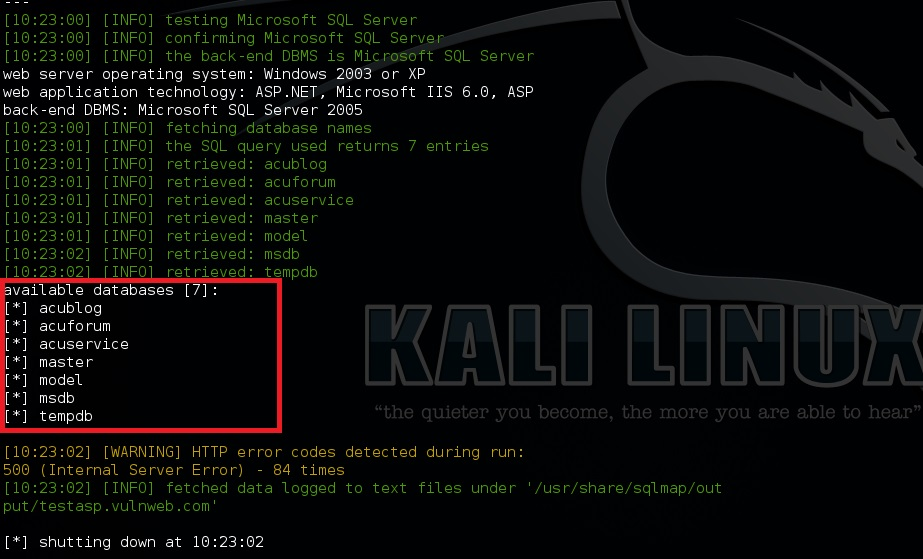
\includegraphics[scale=0.60]{img/SQLDatabasen}
\end{center}
\caption{Beschikbare databasen.}
\label{img:SQLDatabasen}
\end{figure}

Nu kan er een tabel gekozen worden om verder te gaan met het volgende commando om de verschillende soorten tabbellen in die specifieke database op te vragen:
\begin{verbatim} sqlmap -u http://testasp.vulnweb.com/showforum.asp?id=0 -D acuforum 
--tables \end{verbatim}

Zo zijn alle tabbellen zichtbaar en ook hier wordt er weer één uitgekozen om te kijken welke kolommen er precies allemaal in deze tabel zitten:
\begin{verbatim} sqlmap -u http://testasp.vulnweb.com/showforum.asp?id=0 -D acuforum 
-T users --columns \end{verbatim}

Nu kan er al heel veel gedaan worden, nu dat de kolommen zichtbaar zijn, kan er informatie opgevraagd worden uit deze kolommen. In dit geval is het dus mogelijk om de gebruikersnaam en wachtwoord op te vragen:
\begin{verbatim} sqlmap -u http://testasp.vulnweb.com/showforum.asp?id=0 -D acuforum 
-T users -C uname,upass \end{verbatim}

Dit geeft een lijst van 112 velden, zoals te zien is in figuur~\ref{img:SQLData}, want blijkbaar zijn er 112 gebruikers die een account hebben op dit forum. Het is nu mogelijk om al deze gegevens te gebruiken om in te loggen op dit forum. De data wordt ook automatisch lokaal opgeslagen, in dit geval is dit in \textit{/usr/share/sqlmap/output/testasp.vulnweb.com}.

\begin{figure}[H]
\begin{center}
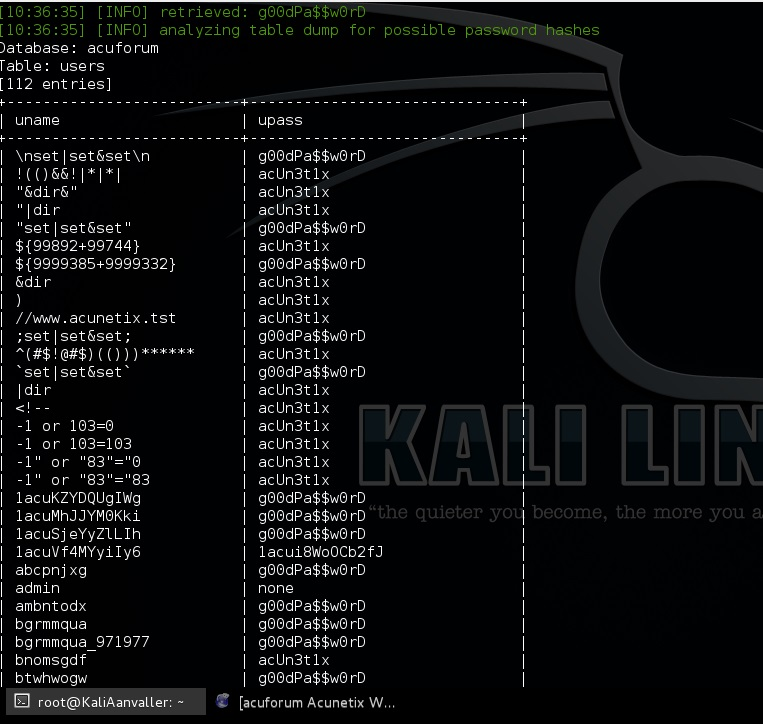
\includegraphics[scale=0.60]{img/SQLData}
\end{center}
\caption{Deel van de uitvoer van SQL-injectie.}
\label{img:SQLData}
\end{figure}

\subsection{Resultaten en beveiliging}
Het spreekt voor zich dat voorgaande aanval een grote catastrofe zou zijn moest dit voorvallen in een eigen ASP.net-webapplicatie. Als een hacker de inloggegevens van gebruikers in handen krijgt kan deze persoonlijke informatie zoals kredietkaartgegevens stelen, maar bij het verkrijgen van een administratorwachtwoord heeft de hacker de touwtjes helemaal in handen. Een goede beveiliging is dus essentieel hier. \newline

Allereerst zouden ontwikkelaars geparameteriseerde queries moeten gebruiken i.p.v. dynamische queries. Hierbij moet de ontwikkelaar alle SQL-code definiëren voordat er parameters doorgegeven worden. Deze manier van coderen zorgt ervoor dat de database het verschil kent tussen code en data. Hierdoor kan een aanvaller de bedoeling van een query niet veranderen, zelfs als deze SQL-commando's toevoegd. \citep{Wichers2013}

Ten tweede is het gebruik van \textit{stored procedures} zeker en vast aan te raden. Deze hebben hetzelfde effect als geparameteriseerde queries, de ontwikkelaar moet ook hier eerst de SQL-code definiëren en daarna worden pas de parameters doorgegeven. Het enige verschil tussen de twee is dat stored procedures in de database worden opgeslagen en dat de webapplicatie ze oproept. Beide technieken zijn goede opties om SQL-injecties tegen te gaan en het is aan de ontwikkelaar om te beslissen welke optie het best in de applicatie past. \citep{Wichers2013}

\section{ARP Spoofing - Man in the middle}
Deze internetlaagaanval kan zeer gevaarlijk zijn omdat het de hacker de mogelijkheid geeft om mee te kijken naar het verkeer dat van een host/server naar de router gaat. Dit kan meekijken met afbeeldingen zijn tot het inkijken van inloggegevens. Hier worden 3 mogelijke Man in the middle-aanvallen uitgeprobeerd om zo tot een oplossing te komen om deze aanval geen kans te geven in een netwerk.

\subsection{Uitvoering}
\subsubsection{Meekijken met slachtoffer}
Om deze aanval uit te voeren staan er best drie terminalvenster open in de Kali Aanvaller-machine zodat er overzichtelijk kan gewerkt worden. In deze aanval wordt het verkeer tussen twee hosts, in dit geval de ADServer met de router (die ook webserver is) onderschept door een derde host die in dit geval de hacker is. Als eerst stap moet er eerst iets nagekeken worden op de Kali-machine en dit gebeurd met volgende lijn:
\begin{verbatim} cat /proc/sys/ipv4/ip_forward \end{verbatim}
Dit zou als uitvoer de waarde 1 moeten geven, indien deze waarde een 0 geeft dan kan dit makkelijk aangepast worden door volgende lijn:
\begin{verbatim} echo 1 >> /proc/sys/net/ipv4/ip_forward \end{verbatim}
Nu dit gedaan is moet de volgende stap gebeuren en dat is de ADServer laten denken dat de aanvallersmachine de default gateway is en de default gateway laten denken dat de aanvallersmachine de ADServer is. Dit gebeurd met volgende twee lijnen:
\begin{verbatim} sudo arpspoof -i eth0 -t 192.168.1.2 192.168.1.3 \end{verbatim}
\begin{verbatim} sudo arpspoof -i eth0 -t 192.168.1.3 192.168.1.2 \end{verbatim}
Het verkeer dat tussen deze twee zal verzonden worden, zal eerst eens passeren voorbij de aanvallersmachine. Zo kan er bijvoorbeeld gekeken worden naar wat de persoon op ADServer zit te kijken in zijn internetbrowser. Bij het typen van volgende lijn in terminalvenster 3 kan dit gedaan worden: 
\begin{verbatim} sudo driftnet -i eth0 \end{verbatim}
Als de persoon op ADServer nu in google zit te kijken naar afbeeldingen van een tijger, dan kan dit via driftnet bekeken worden op de aanvallersmachine zoals te zien is in figuur~\ref{img:Driftnet}. Bij het klikken op één van de afbeelingen wordt deze lokaal opgeslagen. \citep{Walsh2013}

\begin{figure}[H]
\begin{center}
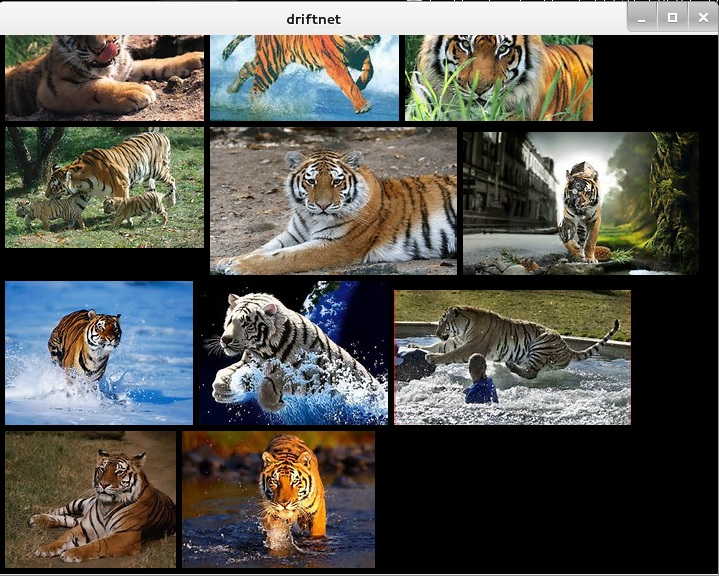
\includegraphics[scale=0.60]{img/Driftnet}
\end{center}
\caption{Aanvaller kijkt mee met persoon op ADServer}
\label{img:Driftnet}
\end{figure}

\subsubsection{HTTP-inloggegevens}
Het bekijken van afbeeldingen is één ding, maar het bekijken van inloggegevens is natuurlijk nog een andere zaak. Via het programma \textit{Ettercap} op de Kali-machine kan er gekeken worden naar inloggegevens van http-website. De werkwijze is als volgt:
\begin{enumerate}
	\item Openen van Ettercap door naar Applicaties - Kali Linux - Sniffing/Spoofing - Network Sniffers - etercap-graphical te gaan.
	\item Kiezen voor Sniff - Unified Snif en de interface selecteren die met het netwerk verbonden is.
	\item Klikken op Hosts - Scan for hosts.
	\item Bij Mitm - ARP Poisining kiezen voor \textit{sniff remote connections}.
	\item Start - Start sniffing om de aanval te starten.
\end{enumerate}
Zoals in figuur~\ref{img:EttercapInlogHTTP} te zien is worden de inloggegevens van een website zonder https getoond in het programma. Deze website is bezocht geweest op de ADServer. \citep{DemmSec2013} 

\begin{figure}[H]
\begin{center}
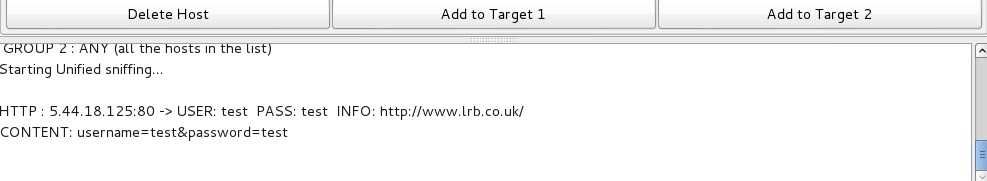
\includegraphics[scale=0.60]{img/EttercapInlogHTTP}
\end{center}
\caption{De inloggegevens van een http-website op ADServer.}
\label{img:EttercapInlogHTTP}
\end{figure}

\subsubsection{HTTPS-inloggegevens}
Met voorgaande techniek zijn HTTPS-wachtwoorden goed beveiligd en dus niet zichtbaar, maar met deze techniek moeten ook deze inloggegevens eraan geloven. Allereerst moet er in het configuratiebestand van Ettercap wat veranderd worden. Bij het openen van het configuratiebestand met volgende lijn code, moet er naar beneden gegaan worden totdat de iptables worden bereikt en moeten 2 lijnen uit commentaar gezet worden zoals te zien is in figuur~\ref{img:EttercapIptables}.
\begin{verbatim} vim /etc/ettercap/etter.conf \end{verbatim}

\begin{figure}[H]
\begin{center}
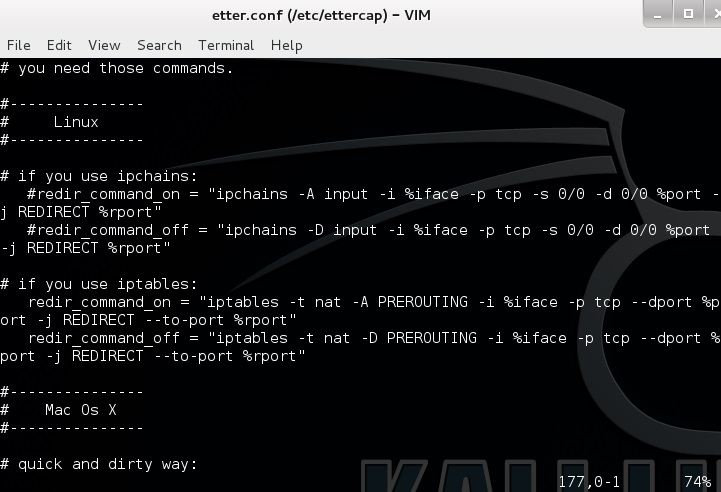
\includegraphics[scale=0.60]{img/EttercapIptables}
\end{center}
\caption{Configuratiebestand zonder iptables in commentaar.}
\label{img:EtterIptables}
\end{figure}

Nu kan er met één lijn een aanval gestart worden in een terminalvenster.
\begin{verbatim} ettercap -TqM ARP:REMOTE /192.168.1.2/ /192.168.1.3/ \end{verbatim}
Dit wil zeggen dat er een Man in the middle aanval met ARP spoofing wordt gestart tussen host 1 (de ADServer met IP 192.168.1.2) en de default gateway (de WebServer met IP 192.168.1.3). Als er nu wordt ingelogged op de ADServer op een website met https-beveiliging om in te loggen, dan worden de inloggegevens toch zichtbaar zoals te zien is in figuur~\ref{img:EttercapInlogHTTPS}. Dit komt doordat de beveiligingscertificaten worden uitgeschakeld door deze aanval. Voordat de aanvaller een website bezoekt waardat er normaal gezien een beveilingscertificaat voor nodig is, dan zal hij de volgende boodschap zien zoals in figuur~\ref{img:EttercapCertificaat} \citep{Canitank2009}

\begin{figure}[H]
\begin{center}
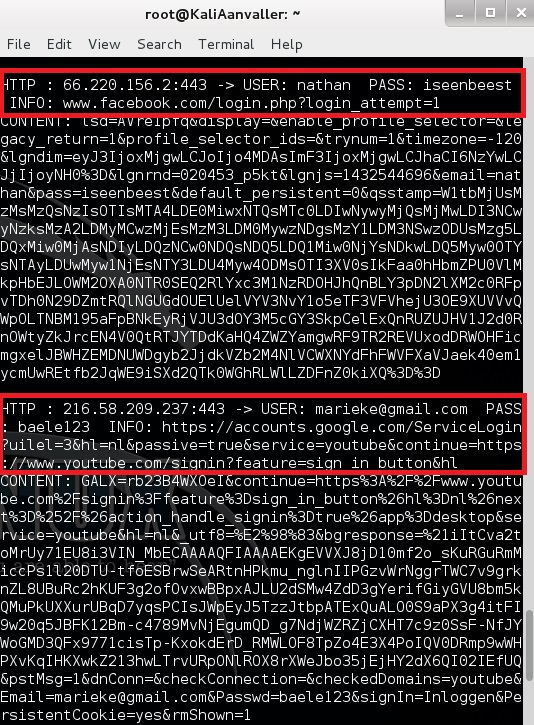
\includegraphics[scale=0.60]{img/EttercapInlogHTTPS}
\end{center}
\caption{De inloggegevens van een https-website op ADServer.}
\label{img:EttercapInlogHTTPS}
\end{figure}

\begin{figure}[H]
\begin{center}
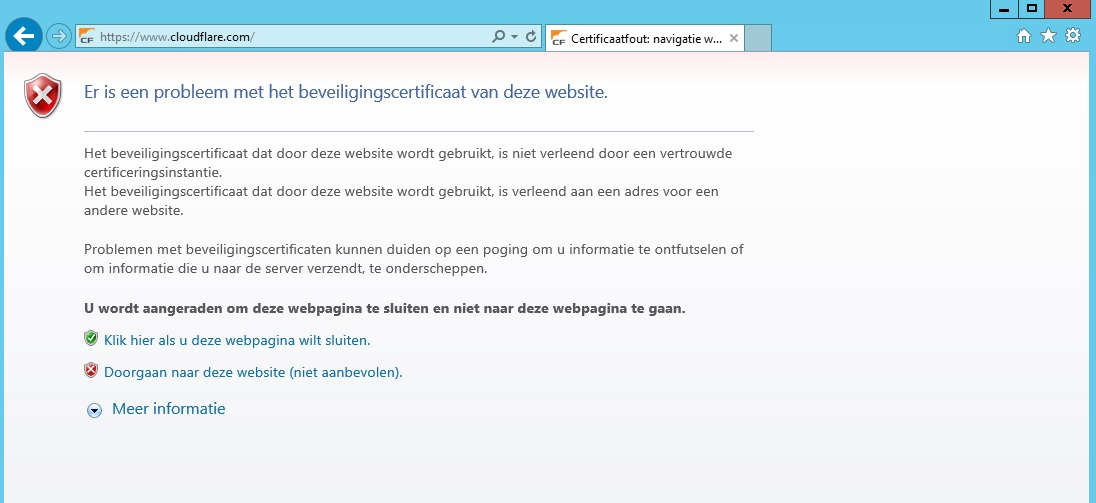
\includegraphics[scale=0.50]{img/EttercapCertificaat}
\end{center}
\caption{De foutboodschap die door de aanval wordt weergeven.}
\label{img:EttercapCertificaat}
\end{figure}

\subsection{Resultaten en beveiliging}
De resultaten van deze aanval vormt de conclusie dat deze inderdaad zeer gevaarlijk is. Het surfgedrag kan niet alleen bekeken worden, maar wachtwoord en inloggegevens van zowal HTTP -en HTTPS-website worden ook doorgegeven aan de aanvaller. Hierdoor is er zeker en vast een aanvulling nodig van de best practices omdat deze duidelijk niet goed genoeg zijn. \newline

Een oplossing om deze soort aanval tegen te werken is het gebruiken van SSL (Secure Socket Layer). Dit is een technology die gebruikt worden om een versleutelde link tussen de server en het browser te maken zodat een soortgelijke aanval niet onopgemerkt kon worden uitgevoerd. Elke keer als er nu een Mitm-aanval plaatsvindt, dan zal er bij het bezoeken van een website met een certificaat nu de foutboodschap van in figuur~\ref{img:EttercapCertificaat} te zien zijn. Indien deze foutboodschap te zien is, dan is het niet aangeraden om verder te gaan en is het beter om gewoon de webpagina te sluiten want dan is de kans groot dat er een aanval plaatsvindt en dat de gegevens kunnen gestolen worden. Tot slot is het gebruik van een VPN (Virtual Private Network) ook een aanrader.

\section{Dictionary attack telnet}
Telnet wordt in het algemeen gezien als onveilig en wordt daarom niet zoveel meer gebruikt. De variant van telnet, genaamd ssh, wordt veel meer gebruikt. Dit voorbeeld kan ook toegepast worden op dezelfde manier bij ssh, het enige verschil is dat het poortnummer van ssh nummer 22 is i.p.v. 23 voor telnet. Bij een portscan kunnen nog andere poorten gebruikt worden om binnen te breken via Hydra, maar in dit geval wordt er gefocussed op telnet.

\subsection{Uitvoering}
Voor deze aanval uit te voeren moeten er in de Kali Aanvaller-machine twee terminalvensters geopend worden. In het eerste venster wordt er gestart met een port scan van het slachtoffer, in dit geval de webserver. Dit wordt gedaan door volgende lijn code in te geven:
\begin{verbatim} nmap 192.168.1.3 \end{verbatim}
Dit is het IP-adres van de webserver en dit zou een lijst moeten weergeven zoals in figuur~\ref{img:PortScan} is te zien. Er is echter maar één waarde belangrijk in deze lijst en dat is poort 23/tcp waar de service TELNET op draait. Dit wil zeggen dat de poort open staat.

\begin{figure}[H]
\begin{center}
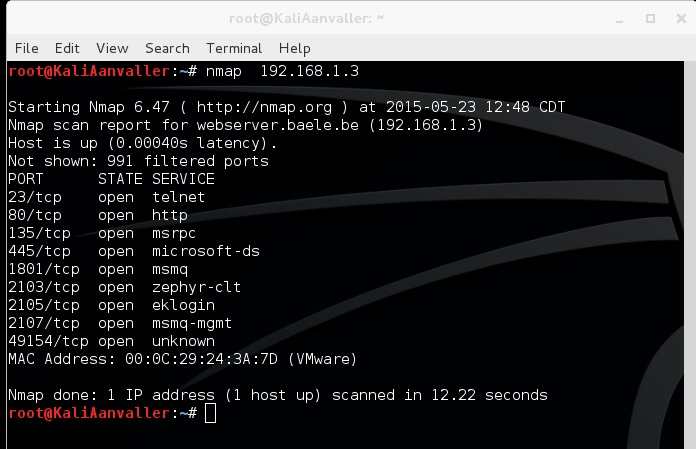
\includegraphics[scale=0.60]{img/HydraPortscan}
\end{center}
\caption{Resultaat van een port scan van de webserver}
\label{img:PortScan}
\end{figure}

In het andere terminalvenster kan nu de hydra-aanval uitgevoerd worden. Dit gebeurt met de volgende lijn:
\begin{verbatim} hydra -t 1 -l Administrator -P /root/test.txt -vV 192.168.1.3 telnet \end{verbatim}
In deze lijn code wordt er de inlognaam van het Administrator-account meegegeven. Standaard is dit \textit{Administrator} maar in de meeste gevallen zal dit een andere naam zijn. Daarna wordt er een bestand meegegeven genaamd test.txt waar er een hele lijst met wachtwoorden in zit. Deze lijst wordt dan volledig overlopen tijdens de aanval. Ten slotte wordt nog het IP-adres van het slachtoffer meegegeven en de service waarmee de aanval zich moet verbinden wat in dit geval \textit{telnet} is. Na het uitvoeren van deze aanval zullen alle mogelijke combinaties geprobeerd worden zoals te zien is in figuur~\ref{img:HydraAanval} en als er een positieve match is tussen gebruikersnaam en wachtwoord dan worden deze in het groen aangetoond zoals in figuur~\ref{img:HydraGeslaagd} te zien is. \citep{Moon2013}

\begin{figure}[H]
\begin{center}
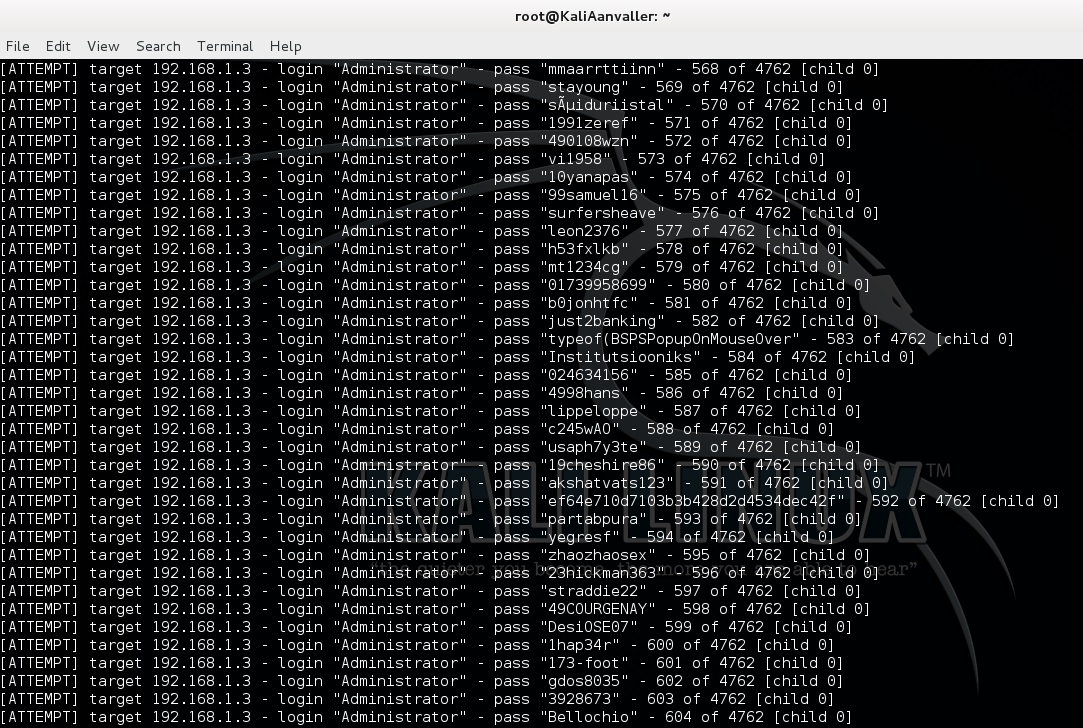
\includegraphics[scale=0.40]{img/HydraAanval}
\end{center}
\caption{Woordenlijst wordt doorlopen.}
\label{img:HydraAanval}
\end{figure}

\begin{figure}[H]
\begin{center}
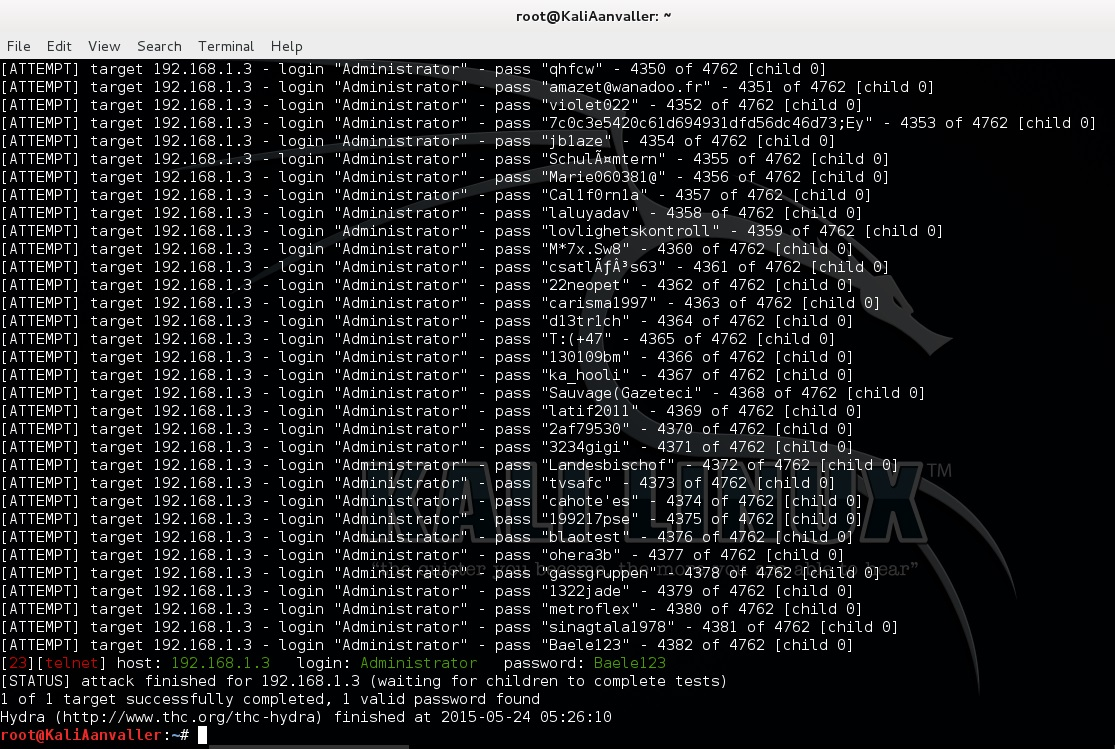
\includegraphics[scale=0.40]{img/HydraGeslaagd}
\end{center}
\caption{Er is een match gevonden.}
\label{img:HydraGeslaagd}
\end{figure}

Hierna kan er met de net verkregen inloggegeven ingelogged worden via het programma \textit{Putty}. Hier wordt er het slachtoffer IP-adres ingevoerd en wordt er gekozen voor poort 23 om daarna de inloggegevens in te vullen. Als deze kloppen dan komt er een verbinding tot stand met het slachtoffer zoals in figuur~\ref{img:HydraPutty} te zien is. Nu heeft de aanvaller volledige controle over de machine.

\begin{figure}[H]
\begin{center}
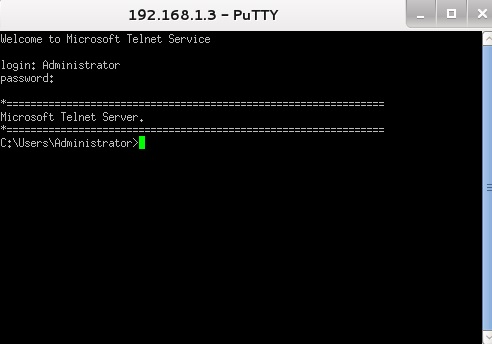
\includegraphics[scale=0.80]{img/HydraPutty}
\end{center}
\caption{Toegang tot de server via putty.}
\label{img:Putty}
\end{figure}

\subsection{Resultaten en beveiliging}
Deze aanval is geslaagd, maar dit is zonder rekening te houden met de best practices. Indien de best practices met betrekking tot het wachtwoord -en accountbeleid van kracht zijn dan heeft deze aanval veel minder kans op slagen. Bij het kiezen van een complex wachtwoord met voldoende tekens zal er veel meer tijd inkruipen om een woordenlijst te doorlopen. Hij het uitschakelen van het administratoraccount en het aanmaken van een nieuw account is er ook al specifieke voorkennis vereist om deze aanval aan te doen of de aanvaller zal moeten gokken. Een woordenlijst met potentiële namen voor een administratoraccount kan eventueel ook toegevoegd worden in dit geval, maar dit neemt ook extra tijd in beslag voor de hacker. Natuurlijk kan er nog een extra best practice worden toegevoegd en dat is om niet onnodige applicatie op de server te installeren. Als telnet of ssh of een ander alternatief nodig zijn, dan zijn de vooropgestelde best practices aan te raden. Indien deze software niet nodig is dan moet deze niet onnodig geïnstalleerd worden, dit geeft een hacker alleen maar mogelijkheden om binnen te breken.


\section{TCP SYN flood}
In deze aanval gaat Sockstress gebruikt worden, dit is één tool die kan gebruikt worden om een TCP SYN flood aanval uit te voeren. Allereerst moet er terug een port scan uitgevoerd worden om te kijken welke poorten er open zijn. Dit zal dezelfde uitvoer hebben als figuur~\ref{img:PortScan}. Alle poorten die hier zichtbaar zijn worden best even ergens genoteerd omdat deze later nog gebruikt zullen worden. Om deze aanval uit te voeren via de Kali Aanvaller-machine moet sockstress eerst gedownload worden aangezien dit niet standaard op Kali Linux staat. Dit wordt gedaan door de volgende lijnen code:
\begin{verbatim} apt-get update \end{verbatim}
\begin{verbatim} apt-get install libpcap0.8 libssl-dev -y \end{verbatim}
\begin{verbatim} wget http://samsclass.info/123/proj10/sockstress-outpost24.tar.gz \end{verbatim}
Indien dit commando niet werkt kan er gegaan worden naar \url{https://defuse.ca/sockstress.htm} waar sockstress ook kan gedownload worden.
\begin{verbatim} tar xzf sockstress-outpost24.tar.gz \end{verbatim}
\begin{verbatim} cd sockstress \end{verbatim}
\begin{verbatim} ./configure \end{verbatim}
\begin{verbatim} nano config.h \end{verbatim}
Met dat laatste lijntje wordt er in het configuratiebestand gegaan en daar moet \textit{\#include <pcap.h>} aangepast worden naar \textit{\#include </usr/include/pcap.h>}. Nu dit is aangepast kan de effectieve aanval worden uitgevoerd. Dit wordt gedaan met volgende lijn code:
\begin{verbatim} ./sockstress -A -c -1 -d 192.168.1.3 -m -1 -Ms -p 23,80,135,445,
1801,2103,2105,2107,49154,49176 -r 100000 -s 192.168.2.0/24 -vv
 \end{verbatim}
Nu kan er naar de webserver gegaan worden om in het taakbeheer te kijken naar de prestaties van het geheugen om te kijken of de aanval is geslaagd. In figuur~\ref{img:SockVoor} is het geheugen te zien voor de aanval en in figuur~\ref{img:SockNa} het geheugen na de aanval. Het geheugen is helemaal volgelopen en er kan niets meer gebeuren op de server, deze moet nu handmatig worden afgesloten.

\begin{figure}[H]
\begin{center}
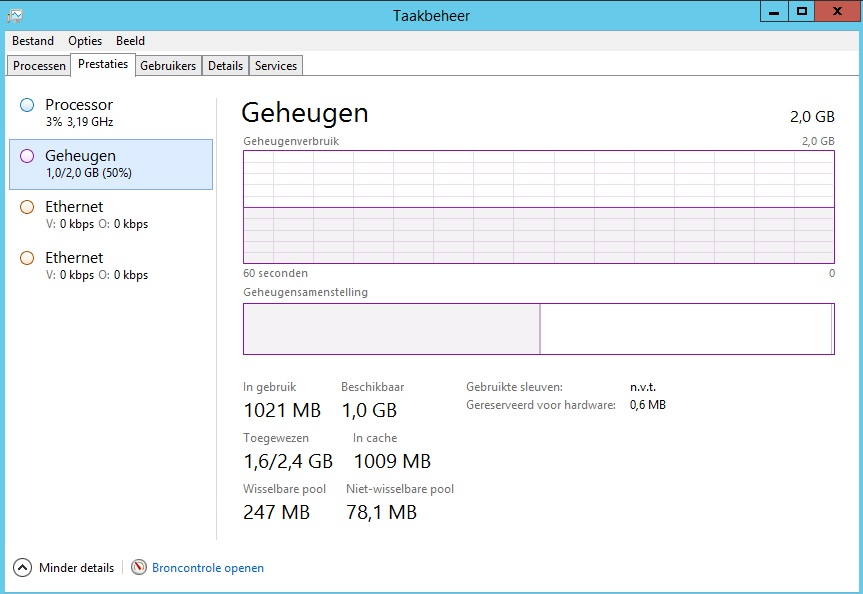
\includegraphics[scale=0.50]{img/SockVoor}
\end{center}
\caption{Gebruikt geheugen voor sockstress-aanval.}
\label{img:SockVoor}
\end{figure}

\begin{figure}[H]
\begin{center}
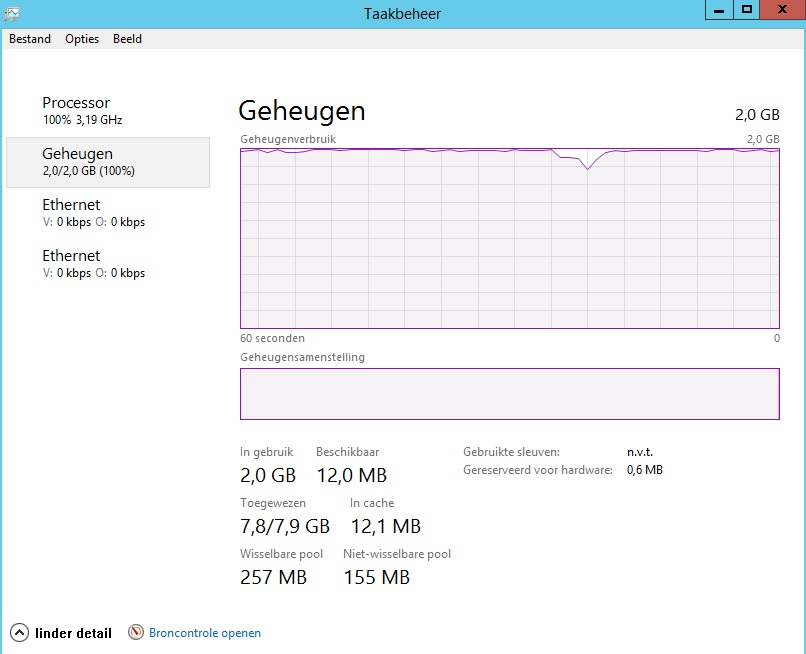
\includegraphics[scale=0.50]{img/SockNa}
\end{center}
\caption{Gebruikt geheugen na sockstress-aanval.}
\label{img:SockNa}
\end{figure}

\subsection{Resultaten en beveiliging}
Het gevolg van deze aanval is dat het RAM-geheugen helemaal is volgelopen zoals te zien is in figuur~\ref{img:SockNa} en dat er op de server niets meer kan gedaan worden. Deze kan ook niet via een remote verbinding worden afgesloten, dit moet effectief handmatig gebeuren. Indien de server een virtuele machine is dan moet er op \textit{Power Off} geklikt worden. Dit kan ervoor zorgen dat alle niet opgeslagen zaken verloren gaan.

Een mogelijke oplossing is het configureren van een Cisco ASA-firewall waarin er regels worden opgesteld waardoor er maar maximum een aantal verbindingen mogelijk zijn. In het terminalvenster van de ASA-firewall worden de volgende lijnen uitgevoerd:
\begin{verbatim} access-list To-Server permit tcp any host 192.168.1.3 \end{verbatim}
Bovenstaande lijn maakt een ACL om het verkeer dat naar de server gaat te identificeren.
\begin{verbatim} class-map Traffic-to-webserver \end{verbatim}
Deze lijn in combinatie met volgende 2 lijnen maakt een class map aan die de ACL oproept. 
\begin{verbatim} match access-list TO-Server \end{verbatim}
\begin{verbatim} exit \end{verbatim}
Nu kan er een policy map aangemaakt worden die als er verkeer voldoet aan de class-map de sessielimiet op 5 zet. Dit wil zeggen dat er dan maar 5 sessies mogelijk zijn.
\begin{verbatim} policy-map global_policy
class Traffic-to-webserver
set connection embryonic-conn-max 5
exit
exit \end{verbatim}
Nu is zijn er maximaal 5 half-open tcp-verbindingen mogelijk en kan een TCP SYN FLOOD-aanval niet meer voorvallen! Bij een aanval zijn er nu maximaal 5 openstaande verbindingen zoals te zien is in figuur~\ref{img:SockOplossing}

\begin{figure}[H]
\begin{center}
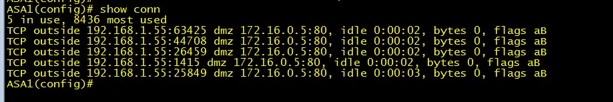
\includegraphics[scale=0.70]{img/SockOplossing}
\captionsource{Maximaal 5 actieve verbindingen bij een aanval.}{https://www.youtube.com/watch?v=AqY3UxXyQTY}
\label{img:SockOplossing}
\end{center}
\end{figure}

\chapter{Conclusie}
\label{ch:conclusie}

% TODO: Trek een duidelijke conclusie, in de vorm van een antwoord op de
% onderzoeksvra(a)g(en). Reflecteer kritisch over het resultaat. Zijn er
% zaken die nog niet duidelijk zijn? Heeft het ondezoek geleid tot nieuwe
% vragen die uitnodigen tot verder onderzoek?
Er kan geconcludeerd worden dat van de vier aanvallen met de hoogste risicofactor er maar één goed kan tegengehouden worden door de best practices die eerder geïmplementeerd zijn en dat is de Hydra-aanval. Bij de andere drie aanvallen zijn er extra maatregelen die moeten worden genomen om de webserver te beschermen tegen deze soort aanvallen. \newline

Bij een SQL-injectie ligt de verantwoordelijkheid vooral bij de ontwikkeleraars en niet echt bij de netwerkbeheerders. De ontwikkelaars moeten ervoor zorgen dat hun code foutvrij en goed gemaakt is. Dit kan met behulp van geparameteriseerde queries of het gebruik van stored procedures. Beide technieken zijn een goede manier om de ASP.net-applicatie die draait op de server te beschermen tegen SQL-injecties. Bij een Man in the middle-aanval is er ook een extra maatregel nodig. De huidige best practices zijn hier ook niet voldoende en hier wordt er best een SSL en/of VPN gebruikt om er zo voor te zorgen dat het duidelijk is wanneer er een aanval plaatsvindt en wanneer niet. Een Sockstress-aanval geraakt ook probleemloos door de best practices en een eventuele oplossing die hier kan gehanteerd worden is het plaatsen en configureren van een Cisco ASA-firewall waardat de configuratie ervoor zorgt dat er maar maximaal 5 openstaande verbindingen kunnen zijn waardoor ook deze aanval geen kans heeft. \newline

Er kan dus gezegd worden dat dit onderzoek een betere kijk geeft over welke aanvallen er relevant zijn voor een webserver met een ASP.net-applicatie en hoe iemand zich hiertegen kan beschermen. Het onderzoek leidt wel tot enkele nieuwe vragen die verder onderzoek niet uitsluiten. Zijn er manieren om rond deze verbeterde best practices te werken? Zijn dit wel de beste oplossingen voor budgetbeperkte ondernemingen? 




\bibliographystyle{apa}
\bibliography{NathanBP}

%%---------- Back matter -------------------------------------------------

\listoffigures
\listoftables

\end{document}
